% =====================================================================
%  EnergyMind Tunisia -- Phase 1 Project Proposal (full)
%  Scope, objectives, data / anomaly-simulation plan, and the preliminary
%  design of each of the four Challenge Goals.
%
%  parts/goal1.tex, goal2.tex, goal4.tex and bibliography.tex are generated
%  from the goal reports by build_parts.py; goal3_condensed.tex and the other
%  parts are written by hand.
%  Build:  python build_parts.py && pdflatex proposal.tex && pdflatex proposal.tex
% =====================================================================
\documentclass[11pt,a4paper]{article}
\usepackage[utf8]{inputenc}
\usepackage[T1]{fontenc}
\usepackage{lmodern}
\usepackage[margin=2.3cm]{geometry}
\usepackage{amsmath,amssymb,mathtools}
\usepackage{booktabs,tabularx,array,multirow}
\usepackage[table]{xcolor}
\usepackage{tikz}
\usetikzlibrary{arrows.meta,positioning,fit,backgrounds,shapes.geometric,calc}
\usepackage{pgfplots}
\pgfplotsset{compat=1.18}
\usepgfplotslibrary{groupplots}
\usepackage{listings}
\usepackage{enumitem}
\usepackage{float}
\usepackage{needspace}
\usepackage{caption}
\usepackage{subcaption}
\usepackage[hidelinks]{hyperref}
\usepackage{bookmark}

% ---------- layout
\newcolumntype{L}{>{\raggedright\arraybackslash}X}
\newcolumntype{Y}{>{\raggedright\arraybackslash}X}
\setlist{itemsep=2pt,topsep=3pt}
\setlength{\emergencystretch}{3em}
\renewcommand{\_}{\textunderscore\allowbreak}
\lstset{basicstyle=\ttfamily\footnotesize,breaklines=true,frame=single,
        columns=fullflexible,keepspaces=true,backgroundcolor=\color{black!3},
        xleftmargin=2pt,xrightmargin=2pt}
\newtheorem{proposition}{Proposition}

% ---------- shared names
\newcommand{\code}[1]{\texttt{#1}}
\providecommand{\GE}{\texttt{GENUINE\_EVENT}}
\providecommand{\MF}{\texttt{METER\_FAULT}}
\providecommand{\SD}{\texttt{SUSPICIOUS\_DATA}}
\providecommand{\ND}{\texttt{NO\_DATA}}
\providecommand{\NORM}{\texttt{NORMAL}}
\newcommand{\lvl}[1]{\textsf{#1}}

% ---------- house palette: every colour name used by the four goal reports is an alias of it
\definecolor{pal-navy}{RGB}{30,58,95}
\definecolor{pal-teal}{RGB}{15,118,110}
\definecolor{pal-orange}{RGB}{230,135,30}
\definecolor{pal-red}{RGB}{190,50,40}
\definecolor{pal-purple}{RGB}{120,60,140}
\definecolor{pal-light}{RGB}{242,244,247}
% the base names used in the Goal 2-4 diagrams (blue!6, green!12, violet!7, ...)
\colorlet{blue}{pal-navy}\colorlet{green}{pal-teal}\colorlet{teal}{pal-teal}
\colorlet{red}{pal-red}\colorlet{orange}{pal-orange}\colorlet{violet}{pal-purple}
% overview figure
\colorlet{c1}{pal-orange}\colorlet{c2}{pal-teal}\colorlet{c3}{pal-navy}\colorlet{c4}{pal-purple}
% Goal 1
\colorlet{mzteal}{pal-teal}\colorlet{mzorange}{pal-orange}\colorlet{mzred}{pal-red}\colorlet{mznavy}{pal-navy}
\colorlet{good}{pal-teal!30}\colorlet{fair}{pal-orange!30}\colorlet{poor}{pal-red!22}
% Goal 4
\colorlet{emblue}{pal-navy}\colorlet{emgreen}{pal-teal}\colorlet{emorange}{pal-orange}
\colorlet{emgrey}{pal-light}\colorlet{emred}{pal-red}

% ---------- tables and captions: booktabs, shaded header row, caption above tables, below figures
\renewcommand{\arraystretch}{1.15}
\setlength{\aboverulesep}{0pt}\setlength{\belowrulesep}{0pt}
\setlength{\extrarowheight}{1.5pt}
\captionsetup{font=small,labelfont={bf,color=pal-navy},labelsep=period}
\captionsetup[table]{position=top,skip=4pt}
\captionsetup[figure]{position=bottom,skip=6pt}

% ---------- Goal 1 helpers (heat cells, plot styles, generated numbers)
\newcommand{\hc}[1]{\expandafter\hcaux\expandafter{\the\numexpr #1*8/10\relax}{#1}}
\newcommand{\hcaux}[2]{\cellcolor{mzteal!#1}\ifnum #2>55 \textcolor{white}{#2}\else #2\fi}
\pgfplotsset{
  mz/.style={width=4.3cm,height=3.4cm,tick label style={font=\tiny},
    label style={font=\scriptsize},title style={font=\scriptsize\bfseries},
    grid=major,grid style={black!10},xmin=0,xmax=72,xtick={0,24,48,72}},
  colormap/ifmap/.style={colormap={ifmap}{rgb255=(255,248,238) rgb255=(245,190,120)
    rgb255=(230,135,30) rgb255=(200,80,30) rgb255=(150,40,30)}},
  colormap/svmmap/.style={colormap={svmmap}{rgb255=(150,40,30) rgb255=(200,80,70)
    rgb255=(255,255,255) rgb255=(120,200,185) rgb255=(15,118,110)}},
}
% generated by gen.py -- do not edit
\newcommand{\zOrd}{1.6, 3.1, 4.0, 4.9}
\newcommand{\zRob}{4.2, 7.7, 9.9, 12.0}
\newcommand{\zOrdHidden}{1}
\newcommand{\cusumAlarm}{84}
\newcommand{\cusumDelay}{4}
\newcommand{\ifOutMin}{0.63}
\newcommand{\ifOutMax}{0.77}
\newcommand{\ifNormMean}{0.46}
\newcommand{\ifSMin}{0.40}
\newcommand{\ifSMax}{0.80}
\newcommand{\pathNormal}{11.6}
\newcommand{\pathAnom}{5.2}

% generated by n1_experiment.py -- do not edit
\newcommand{\nOneDays}{10{,}715}
\newcommand{\nOneClean}{9{,}494}
\newcommand{\nOneEvents}{74}
\newcommand{\stackFPR}{2.3}
\newcommand{\gapSd}{0.6}
\newcommand{\balFPR}{5.2}
\newcommand{\nRare}{16}
\newcommand{\nRareHit}{9}


% ---------- Goal 4 helpers
\newcommand{\TODO}[1]{\textcolor{emred}{\textbf{[TODO: #1]}}}
\newcommand{\impl}{\textcolor{emgreen}{\textsc{impl}}}
\newcommand{\design}{\textcolor{emorange}{\textsc{design}}}
\newcommand{\hdr}{\rowcolor{pal-navy!12}}

\title{\textbf{EnergyMind Tunisia}\\[3pt]\large Phase 1 Project Proposal\\[2pt]
\normalsize Trustworthy monitoring of a smart-metered neighbourhood: telling grid events from bad data}
\author{}
\date{IEEE TSYP14 --- PES $\times$ IES Challenge \quad$\cdot$\quad 15 October 2026}

\begin{document}
\maketitle
\begin{abstract}
\noindent A smart meter that reports something surprising is telling one of two stories: either the
\emph{grid} did something unusual (an outage, a voltage sag, a demand surge) or the \emph{data} is wrong (a
drifting sensor, a corrupted value, a bypassed or falsified meter). The two need opposite responses, and
confusing them is costly. We propose a human--AI system for a smart-metered low-voltage neighbourhood that
(1) detects anomalous and biased readings with a hybrid of physics rules, statistics and unsupervised
learning, (2) explains each verdict with a calibrated confidence and an auditable record, (3) routes every
case to the right level of human control, never letting confidence override consequence, and (4) lets
several neighbourhoods learn from each other without sharing raw readings. Phase~1 delivers a labelled,
Tunisia-calibrated simulated dataset, the design of all four goals, and a first detection prototype run on
one neighbourhood: at 2.3\% false positives it detects 30 of 36 genuine events, 23 of 30 meter faults and
6 of 8 falsifications, and it shows plainly which cases remain hard.
\end{abstract}

\tableofcontents
\newpage

\section{Scope}
\label{sec:scope}

\paragraph{The slice of the energy system we monitor.} The low-voltage distribution network of a
smart-metered residential neighbourhood, from the secondary of the MV/LV transformer to the customer meters:
\begin{itemize}
  \item \textbf{Customer smart meters} reporting every 30~minutes: imported energy, PV export, reactive energy,
        mean/min/max voltage, current, power factor, voltage distortion and an event log.
  \item \textbf{One accurate meter at the head of each feeder}, which sees the true energy flow and the
        feeder voltage. It makes two physical cross-checks possible: the feeder energy balance (head minus the
        sum of customer meters) and the comparison of each meter's voltage with the head's.
  \item \textbf{Context}: weather (temperature, irradiance), calendar (weekends, Tunisian public holidays,
        Ramadan) and the static description of each meter and home.
\end{itemize}

\paragraph{Single-node prototype and multi-node design.} Our simulated dataset contains three such
neighbourhoods (\emph{nodes}) with different climates and customer mixes (Table~\ref{tab:nodes}). As the
challenge requires, Goals~1--3 are prototyped on a single node, \textbf{N1} (coastal suburb: one transformer,
30 meters on three feeders of 10, three homes with rooftop PV). Goal~4 connects N1, N2 and N3; multi-node
sharing is a documented design in Phase~1, as the challenge allows.

\begin{table}[H]
\centering\small
\caption{Nodes of the simulated dataset (60 meters, 7 feeders, year 2025).}
\label{tab:nodes}
\begin{tabularx}{\textwidth}{@{}l >{\raggedright\arraybackslash}p{4.4cm} r r L@{}}
\toprule\hdr
\textbf{Node} & \textbf{Profile} & \textbf{Meters} & \textbf{Feeders} & \textbf{Role} \\
\midrule
N1 & Coastal suburb & 30 & 3 & Phase 1 prototype (Goals 1--3); sharing participant \\
N2 & Hot interior town & 15 & 2 & Sharing participant (Goal 4) \\
N3 & Mixed residential / commercial & 15 & 2 & Sharing participant (Goal 4) \\
\bottomrule
\end{tabularx}

\end{table}

\paragraph{The question the system answers.} For every suspicious reading: \emph{can this data be trusted,
and if not, why, how sure are we, and who should act?} The answer is one of four verdicts shared by all
components --- \NORM, \GE{} (the data is right and the grid did something), \MF{} (a faulty or corrupted
meter) and \SD{} (readings that look manipulated) --- plus \ND{} when readings are missing.

\paragraph{Out of scope.} Control of real STEG equipment (the system recommends; switching and disconnection
always need human approval); the medium- and high-voltage network; real STEG meter data (all data are
simulated and labelled as such); billing and customer-facing processes.

% =====================================================================
\section{Objectives}
\label{sec:objectives}

Each objective is tied to a measurable target. Phase~1 targets are design deliverables and a first measured
baseline; Phase~2 targets are the ones we will report on the full prototype.

\begin{table}[H]
\centering\small
\caption{Objectives and targets.}
\begin{tabularx}{\textwidth}{@{}>{\raggedright\arraybackslash}p{3.3cm}LL@{}}
\toprule\hdr
\textbf{Objective} & \textbf{Phase 1 (this submission)} & \textbf{Phase 2 target (measured on N1)} \\
\midrule
\textbf{O1 Detect} anomalous and biased readings (Goal 1) &
Hybrid detector designed and run on N1: 2.3\% false positives on clean meter-days; 30/36 genuine events, 23/30 meter faults, 6/8 falsifications detected &
Keep false positives $\le$\,2.5\%; detect the physically consistent cases (bypass, bias, drift) now missed, via a modelled feeder-balance residual \\
\addlinespace
\textbf{O2 Explain} each verdict (Goal 2) &
Rule cascade, 4-class calibrated confidence, explanation pipeline and log schema designed &
Brier score and calibration curve per class; $\ge$\,90\% of named channels and scopes correct on labelled events; faithfulness check on every LLM text \\
\addlinespace
\textbf{O3 Govern} human--AI decisions (Goal 3) &
Governance levels, risk model, routing rules, blind-first console and scenarios designed &
Zero unsafe automatic actions; missed-escalation and false-escalation rates against the dataset's reference responses; coverage--accuracy curve \\
\addlinespace
\textbf{O4 Share} knowledge across nodes (Goal 4) &
Four protected channels, privacy accounting, threat model and canary adoption designed &
Detection of attack types a node has never seen, with vs.\ without sharing; privacy--utility curve; corrupted-node test \\
\addlinespace
\textbf{O5 Be honest} about evidence &
Every measured number is printed by code in the repository (\code{scripts/check\_dataset.py} for the data, \code{docs/goal1\_detection/n1\_experiment.py} for detection; the governance scenarios and safety invariants are tests in \code{tests/test\_governance.py}); untested items are labelled as design &
Results reported per event with confidence intervals, never as a single accuracy figure \\
\bottomrule
\end{tabularx}

\end{table}

% =====================================================================
\section{Data and Anomaly-Simulation Plan}
\label{sec:data}

Real fault- and attack-labelled distribution data is rare and is not public for Tunisia, so the project uses a
simulated dataset with exact labels. Full documentation is in the repository's data card
(\code{docs/data\_card.md}).

\subsection{The dataset}
\begin{itemize}
  \item \textbf{One table, one row per meter per half-hour}: 1\,051\,200 rows $\times$ 67 columns; 60 meters on
        7 feeders in 3 nodes; 1~January--31~December 2025, local time. Designed and generated by our team with a fixed random
        seed (2025); the generator in \code{simulate/} (healthy network, anomaly injection, join) reproduces the
        committed file exactly, and every figure quoted from it is printed by \code{scripts/check\_dataset.py}.
  \item \textbf{Column groups}: identifiers; meter measurements (10); meter and home details (21); weather and
        calendar (6); feeder context (11, including feeder-head energy and voltage and the energy-balance gap);
        ground truth (15 columns prefixed \code{gt\_}).
  \item \textbf{Label hygiene}: the \code{gt\_*} columns and two simulator settings are never model inputs; five
        ``oracle'' columns (true energy, true voltage, true losses) are used only to analyse errors.
\end{itemize}

\subsection{How the normal behaviour is generated}
\begin{enumerate}
  \item \textbf{Weather} for three Tunisian climates (coastal, interior, southern coast), with heat waves and
        solar irradiance.
  \item \textbf{Household load} with Saturday--Sunday weekends, public holidays, \textbf{Ramadan} (suhoor and
        iftar peaks), summer vacations, temperature-driven air conditioning, electric heating, and rooftop PV
        with export.
  \item \textbf{Calibration} to public Tunisian figures: residential consumption near the STEG average of about
        1\,450--1\,470~kWh per year (N1: 1\,475~kWh); homes with air conditioning use about $1.68\times$ more in
        July--August than in January--February.
  \item \textbf{Electrical model}: voltage drops along each feeder and rises with PV export; power factor falls
        with air-conditioning load; meters add small measurement noise (energy agrees with
        $V\,I\,\mathrm{PF}\,\Delta t$ within 0.93\% median, 2.7\% at the 95th percentile).
  \item \textbf{Feeder-head meter} seeing true energy plus line losses and unmetered street lighting, which
        creates the realistic $\approx$\,5\% feeder balance gap.
\end{enumerate}

\subsection{How anomalies are injected}
Genuine events are injected first, then data problems and falsification at meter level. Every row is labelled
with its class (\code{gt\_label}), exact cause (\code{gt\_subtype}, 29 values), event identifier
(\code{gt\_event\_id}), whether the data can be trusted, and a suggested response. Rows are labelled only while
the anomaly is visible (a drift once it reaches 1\%, a selective bypass only in the bypassed hours).

\begin{table}[H]
\centering\footnotesize
\caption{Anomaly classes and injection recipes. 93.2\% of rows are normal.}
\label{tab:classes}
\begin{tabularx}{\textwidth}{@{}>{\raggedright\arraybackslash}p{2.3cm}>{\raggedright\arraybackslash}p{1.6cm}L r@{}}
\toprule\hdr
\textbf{Class} & \textbf{Data trusted?} & \textbf{Injected causes (recipe)} & \textbf{Rows} \\
\midrule
\code{grid\_event} & yes, genuine & outage and post-restoration surge; scheduled load shedding (July--August); voltage sag ($-15$ to $-45$~V) and swell; demand surge ($\times1.35$--$1.8$ for 1.5--4~h); cold-load pickup & 0.37\% \\
\code{equipment\_failure} & yes, genuine & cable fault (meters beyond the cut lose supply); transformer degradation ending in a trip & 0.64\% \\
\code{sensor\_fault} & no & gain drift (slow, mostly under-reading); bias step ($\times0.86$--$0.93$ or $\times1.07$--$1.14$ for 3--11 weeks); voltage-sensor offset drift; clock shift (1--3~h); stuck value (3--48~h) & 2.90\% \\
\code{data\_corruption} & no & spike ($\times8$--$40$); sign flip; saturation (99.999); Wh reported as kWh & 0.02\% \\
\code{falsification} & no & \emph{physical}: partial bypass (energy and current $\times0.4$--$0.8$), selective bypass, meter zeroing; \emph{data-only}: scaling ($\times0.3$--$0.75$), evasive random-walk scaling, replay of last week, inflation (framing a neighbour), coordinated attack on three meters & 2.74\% \\
\code{comm\_loss} & no data & all measurements missing for 1.5--48~h (PLC meters most exposed) & 0.10\% \\
\bottomrule
\end{tabularx}

\end{table}

\paragraph{Why detection is deliberately not trivial.} A real event hits neighbours together, a failing sensor
is isolated --- except for the coordinated attack. Physical tampering keeps energy, voltage and current
consistent and only opens the feeder balance; data-only injection breaks that consistency but leaves voltage
untouched. Hard negatives are included on purpose: summer vacations (genuinely low use), the Ramadan shift,
heat-wave surges, PV export reversing the current, and post-outage surges.

\subsection{What the data looks like on the prototype node}
Node N1 has 98 labelled events in 2025: 37 genuine (33 grid events, 4 equipment failures), 33 meter faults (25
corruption, 8 sensor faults), 8 falsifications (one of each type) and 20 communication losses. Two facts shape
the whole design:
\begin{itemize}
  \item \textbf{A supply loss is recorded as zeros, not as missing data} (683 readings in N1), so ``flat at
        zero'' must be read as an outage before it is read as a frozen meter.
  \item \textbf{Rare events are really rare}: each falsification type occurs once in N1 and 2--3 times in the
        whole dataset, at most once per node.
\end{itemize}

\subsection{Evaluation protocol}
A calendar split (train January--August, validate September--October, test November--December) does not work
here: in N1 the last two months contain no falsification and no sensor-bias event. All goals therefore use
\textbf{5-fold cross-validation with folds grouped by event} (no event is split between fitting and testing;
clean days grouped by meter-week), unsupervised models are trained on clean days only, and results are reported
per class and per event with intervals. This protocol is implemented in the repository
(\code{energymind.data.event\_folds}).

\subsection{Known limitations of the data}
The data are synthetic: a detector tuned here may overfit the generator. The anomaly share ($\approx$\,6.8\%) is
higher than in reality so that models have examples. Meter fields follow an assumed IEC-style half-hourly
profile. There is one transformer per node and no three-phase imbalance. All results are reported as simulated.

% =====================================================================

\section{Preliminary Design: Overview}
\label{sec:design}

\begin{figure}[H]
\centering
\resizebox{\textwidth}{!}{%
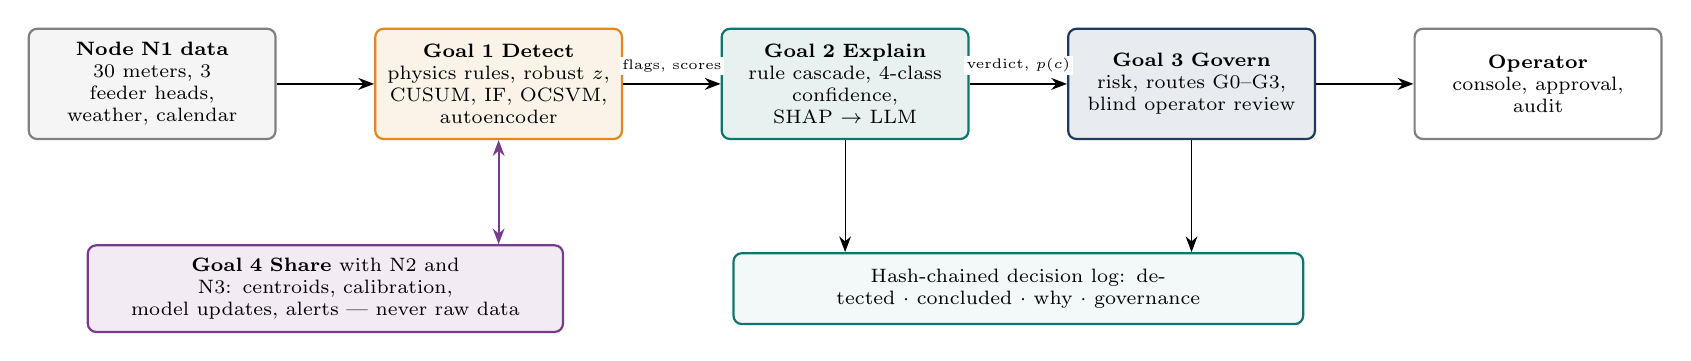
\begin{tikzpicture}[
  b/.style={draw,rounded corners=3pt,align=center,font=\scriptsize,minimum height=14mm,text width=29mm,thick},
  lab/.style={font=\tiny,fill=white,inner sep=1pt},
  >={Stealth[length=2mm]}]
\node[b,draw=black!50,fill=black!4] (m) at (0,0) {\textbf{Node N1 data}\\ 30 meters, 3 feeder heads,\\ weather, calendar};
\node[b,draw=c1,fill=c1!10] (g1) at (4.4,0) {\textbf{Goal 1 Detect}\\ physics rules, robust $z$,\\ CUSUM, IF, OCSVM,\\ autoencoder};
\node[b,draw=c2,fill=c2!10] (g2) at (8.8,0) {\textbf{Goal 2 Explain}\\ rule cascade, 4-class\\ confidence, SHAP $\to$ LLM};
\node[b,draw=c3,fill=c3!10] (g3) at (13.2,0) {\textbf{Goal 3 Govern}\\ risk, routes G0--G3,\\ blind operator review};
\node[b,draw=black!50,fill=white] (op) at (17.6,0) {\textbf{Operator}\\ console, approval,\\ audit};
\node[b,draw=c2,fill=c2!5,text width=70mm,minimum height=9mm] (log) at (11.0,-2.6) {Hash-chained decision log: detected $\cdot$ concluded $\cdot$ why $\cdot$ governance};
\node[b,draw=c4,fill=c4!10,text width=58mm,minimum height=11mm] (g4) at (2.2,-2.6) {\textbf{Goal 4 Share} with N2 and N3: centroids, calibration,\\ model updates, alerts --- never raw data};
\draw[->,thick] (m)--(g1);
\draw[->,thick] (g1)--node[lab,above=1mm]{flags, scores}(g2);
\draw[->,thick] (g2)--node[lab,above=1mm]{verdict, $p(c)$}(g3);
\draw[->,thick] (g3)--(op);
\draw[->] (g2.south)--(g2.south|-log.north); \draw[->] (g3.south)--(g3.south|-log.north);
\draw[<->,thick,c4] (g1.south)--(g1.south|-g4.north);
\end{tikzpicture}}
\caption{System overview on one node. Sections~\ref{g1-sec:goal1}--\ref{g4-sec:goal4} give the preliminary design of each goal; Goal~3 is condensed here, its complete design is in \code{docs/goal3\_governance}.}
\label{fig:overview}
\end{figure}


\clearpage
% generated by build_parts.py from the goal report -- edit the report, not this file
\section{Goal 1: Anomaly and Bias Detection}
\label{g1-sec:goal1}
\paragraph{Summary.} Our system must decide, for every suspicious reading, whether the \emph{grid}
did something unusual or the \emph{data} is wrong, because the two need opposite responses. No single
detector can do this. We therefore combine (i) physics and statistical rules, which are auditable,
(ii) three unsupervised machine-learning detectors trained only on clean data, which are sensitive to subtle
patterns, and (iii) a cross-sensor consistency reasoner that separates genuine events from data-quality
problems. Section~\ref{g1-sec:stack} tests the detection layers on node N1 of the EnergyMind dataset and
reports, per fault type, what they catch and what they still miss.

% =====================================================================
\subsection{The Problem: a Suspicious Number Has Two Possible Meanings}
\label{g1-sec:problem}
An anomaly is a pattern that deviates from expected behaviour~\cite{chandola}. In our prototype node (N1 of
the EnergyMind dataset: one transformer, 30 smart meters on 3 low-voltage feeders of 10, three homes with
rooftop PV, readings every 30~minutes, each feeder metered at its head) a surprising value can come from the
\textbf{grid} or from
the \textbf{data chain}, and the right response differs: a real event needs operational action, a faulty or
falsified sensor needs to be distrusted and repaired. A further difficulty is that an informed attacker can
craft false data that passes standard bad-data checks~\cite{fdi}, so one test is never enough.

\begin{figure}[H]
\centering
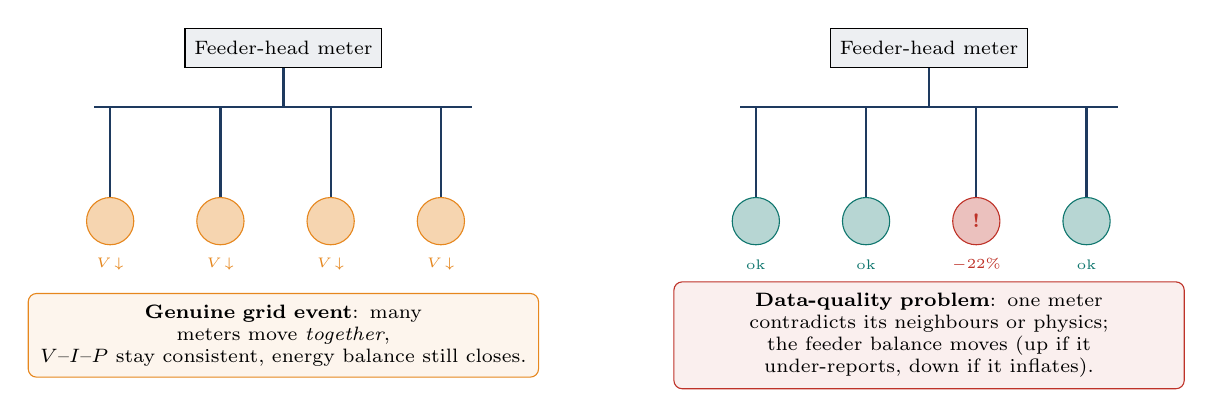
\begin{tikzpicture}[
  meter/.style={circle,draw,minimum size=6mm,inner sep=0pt,font=\scriptsize\bfseries},
  head/.style={draw,fill=mznavy!8,font=\scriptsize,minimum height=5mm},
  note/.style={draw,rounded corners=3pt,font=\scriptsize,align=center,text width=62mm,inner sep=4pt}]
\foreach \side/\x in {L/0,R/8.2}{
  \node[head] (h\side) at (\x+3,2.2) {Feeder-head meter};
  \draw[mznavy,thick] (h\side.south)--(\x+3,1.45);
  \draw[mznavy,thick] (\x+0.6,1.45)--(\x+5.4,1.45);
}
\foreach \x in {0.8,2.2,3.6,5.0}{\draw[mznavy,thick] (\x,1.45)--(\x,0.3);}
\foreach \x in {9.0,10.4,11.8,13.2}{\draw[mznavy,thick] (\x,1.45)--(\x,0.3);}
% left: genuine event, every meter sees the same voltage dip
\foreach \x in {0.8,2.2,3.6,5.0}{
  \node[meter,fill=mzorange!35,draw=mzorange] at (\x,0) {};
  \node[font=\tiny,text=mzorange] at (\x,-0.55) {$V\!\downarrow$};}
% right: data-quality problem on a single meter
\foreach \x in {9.0,10.4,13.2}{
  \node[meter,fill=mzteal!30,draw=mzteal] at (\x,0) {};
  \node[font=\tiny,text=mzteal] at (\x,-0.55) {ok};}
\node[meter,fill=mzred!30,draw=mzred,text=mzred] at (11.8,0) {!};
\node[font=\tiny,text=mzred] at (11.8,-0.55) {$-22\%$};
\node[note,fill=mzorange!8,draw=mzorange] at (3,-1.45)
  {\textbf{Genuine grid event}: many meters move \emph{together},\\ $V$--$I$--$P$ stay consistent, energy balance still closes.};
\node[note,fill=mzred!8,draw=mzred] at (11.2,-1.45)
  {\textbf{Data-quality problem}: one meter contradicts its neighbours or physics;\\ the feeder balance moves (up if it under-reports, down if it inflates).};
\end{tikzpicture}
\caption{The core question. Left: a real event is visible on many sensors and obeys physics. Right: a faulty
or falsified channel disagrees with redundant measurements. This cross-sensor logic is the backbone of our
design.}
\label{g1-fig:core}
\end{figure}

% =====================================================================
\subsection{Types of Anomalies}
\label{g1-sec:types}
The literature classifies anomalies by how they relate to context~\cite{chandola}. We use that
classification and map it onto grid failures (Figure~\ref{g1-fig:types}, Table~\ref{g1-tab:taxonomy}).

\begin{figure}[H]
\centering
\begin{tikzpicture}
\begin{groupplot}[group style={group size=4 by 1,horizontal sep=7mm},mz,xlabel={hours}]
\nextgroupplot[title={Point},ylabel={$V$},ymin=225,ymax=249]
  \addplot[black!35,thin] table[x=t,y=v]{../goal1_detection/data/types_point.dat};
  \addplot[mzred,only marks,mark=diamond*,mark size=2pt] table[x=t,y=anom]{../goal1_detection/data/types_point.dat};
  \addplot[mzred,only marks,mark=diamond*,mark size=2pt] table[x=t,y=ref]{../goal1_detection/data/types_point.dat};
\nextgroupplot[title={Contextual},ymin=225,ymax=249]
  \addplot[black!35,thin,unbounded coords=jump] table[x=t,y=v]{../goal1_detection/data/types_context.dat};
  \addplot[mzred,only marks,mark=*,mark size=1.6pt] table[x=t,y=anom]{../goal1_detection/data/types_context.dat};
  \draw[mzred,thick,-{Stealth[length=1.5mm]}] (axis cs:27,227.3)--(axis cs:27,231.6);
\nextgroupplot[title={Collective (stuck)},ymin=225,ymax=249]
  \addplot[black!35,thin,unbounded coords=jump] table[x=t,y=v]{../goal1_detection/data/types_stuck.dat};
  \addplot[mzred,thick,const plot,unbounded coords=jump] table[x=t,y=anom]{../goal1_detection/data/types_stuck.dat};
\nextgroupplot[title={Collective (drift)},ymin=225,ymax=244]
  \addplot[black!35,thin] table[x=t,y=v]{../goal1_detection/data/types_drift.dat};
  \addplot[mzorange,thick,unbounded coords=jump] table[x=t,y=anom]{../goal1_detection/data/types_drift.dat};
\end{groupplot}
\end{tikzpicture}
\caption{Illustrative voltage traces (synthetic, 30-min samples as in the dataset). Grey: normal behaviour. Red/amber: the
anomaly. A \emph{point} anomaly is one odd value; a \emph{contextual} anomaly is a value that is normal in
general but wrong for its time of day; \emph{collective} anomalies are odd only as a sequence (a frozen
sensor, a slow drift).}
\label{g1-fig:types}
\end{figure}

\begin{table}[H]
\centering
\caption{From anomaly types to the fault types of the EnergyMind dataset. Genuine events are \emph{expected} to
trigger the detectors; the reasoner (Section~\ref{g1-sec:stack}) must not call them bad data. Missing readings
(communication loss) are not scored: they are passed on as ``no data''.}
\label{g1-tab:taxonomy}
\small
\begin{tabularx}{\textwidth}{@{}>{\raggedright\arraybackslash}p{3.1cm}>{\raggedright\arraybackslash}p{2.3cm}LL@{}}
\toprule\hdr
\textbf{Project anomaly} & \textbf{Type~\cite{chandola}} & \textbf{Signature in the data} & \textbf{First line of defence} \\
\midrule
Impossible value (spike, sign or unit error, saturation) & Point & $E<0$, $E=99.999$, $\times1000$, $\times8$--$40$ & Range rules \\
Stuck meter & Collective & Every channel frozen ($E$ \emph{and} $V$) & Flat-line rule \\
Data-only injection (scale, evasion, inflate, coordinated) & Contextual & $E \neq V I \cos\varphi\,\Delta t$ & Physics rule (skipped while exporting) \\
Replay & Collective & Same half-hour one week earlier & Profile residual, ML ensemble \\
Voltage sensor offset & Collective & Meter $V$ persistently \emph{above} feeder-head $V$ & $V$-vs-head rule, CUSUM \\
Sensor bias, gain drift ($\pm$2--14\%) & Collective & $V$, $I$, $E$ scaled together: physics holds & Feeder balance (feeder level), profile, ML \\
Physical bypass, zeroing & Contextual & Energy \emph{and} current reduced: physics holds & Feeder balance, zero-run, ML \\
Clock shift & Collective & All channels delayed 1--3~h & Lag correlation with profile \\
\midrule
\emph{Genuine} outage, sag, swell, surge, cable fault & (not an error) & Many meters, physics holds; $V=0$ on supply loss & Flagged here; classified by the reasoner \\
\bottomrule
\end{tabularx}

\end{table}

% =====================================================================
\subsection{Families of Detection Methods and Our Choice}
\label{g1-sec:families}
Methods can be organised by \emph{what knowledge they use} and by \emph{how many labels they
need}~\cite{chandola,pang}. Because labelled faults are rare in grids, we are driven toward the
semi-supervised and unsupervised regimes: learn what ``normal'' looks like from clean data, and flag
deviations (Figure~\ref{g1-fig:taxonomy}).

\begin{figure}[H]
\centering
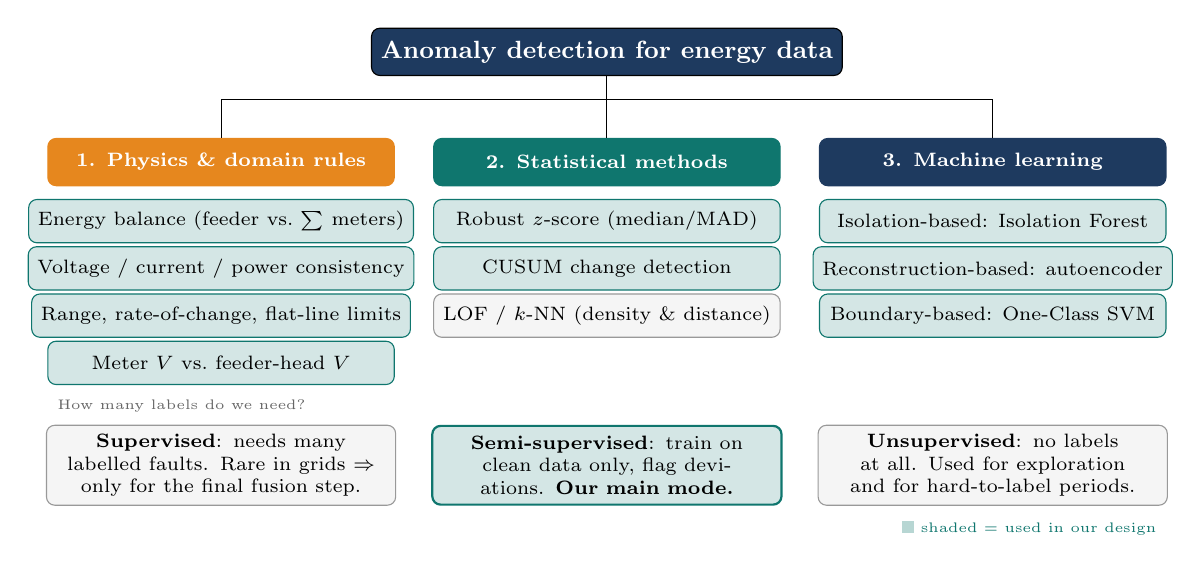
\begin{tikzpicture}[
  fam/.style={draw,rounded corners=3pt,text=white,font=\scriptsize\bfseries,minimum width=44mm,minimum height=6mm},
  used/.style={draw=mzteal,fill=good!60,rounded corners=3pt,font=\scriptsize,minimum width=44mm,minimum height=5.5mm},
  unused/.style={draw=black!40,fill=black!4,rounded corners=3pt,font=\scriptsize,minimum width=44mm,minimum height=5.5mm},
  lab/.style={draw,rounded corners=3pt,font=\scriptsize,align=center,text width=42mm,minimum height=10mm}]
\node[fam,fill=mznavy,minimum width=44mm,font=\small\bfseries] (root) at (4.9,1.4) {Anomaly detection for energy data};
\node[fam,fill=mzorange,draw=mzorange] (f1) at (0,0) {1. Physics \& domain rules};
\node[fam,fill=mzteal,draw=mzteal] (f2) at (4.9,0) {2. Statistical methods};
\node[fam,fill=mznavy,draw=mznavy] (f3) at (9.8,0) {3. Machine learning};
\draw (root.south)--(4.9,0.8); \draw (0,0.8)--(9.8,0.8);
\foreach \f in {f1,f2,f3}{\draw (\f.north|-0,0.8)--(\f.north);}
\node[used] at (0,-0.75) {Energy balance (feeder vs.\ $\sum$ meters)};
\node[used] at (0,-1.35) {Voltage / current / power consistency};
\node[used] at (0,-1.95) {Range, rate-of-change, flat-line limits};
\node[used] at (0,-2.55) {Meter $V$ vs.\ feeder-head $V$};
\node[used] at (4.9,-0.75) {Robust $z$-score (median/MAD)};
\node[used] at (4.9,-1.35) {CUSUM change detection};
\node[unused] at (4.9,-1.95) {LOF / $k$-NN (density \& distance)};
\node[used] at (9.8,-0.75) {Isolation-based: Isolation Forest};
\node[used] at (9.8,-1.35) {Reconstruction-based: autoencoder};
\node[used] at (9.8,-1.95) {Boundary-based: One-Class SVM};
\node[font=\tiny,anchor=west,text=black!60] at (-2.2,-3.1) {How many labels do we need?};
\node[lab,draw=black!40,fill=black!4] at (0,-3.85) {\textbf{Supervised}: needs many labelled faults. Rare in grids $\Rightarrow$ only for the final fusion step.};
\node[lab,draw=mzteal,fill=good!60,thick] at (4.9,-3.85) {\textbf{Semi-supervised}: train on clean data only, flag deviations. \textbf{Our main mode.}};
\node[lab,draw=black!40,fill=black!4] at (9.8,-3.85) {\textbf{Unsupervised}: no labels at all. Used for exploration and for hard-to-label periods.};
\node[font=\tiny,text=mzteal,anchor=east] at (12,-4.65) {\textcolor{good}{\rule{1.5mm}{1.5mm}} shaded = used in our design};
\end{tikzpicture}
\caption{Taxonomy of detectors. Teal boxes are the methods we use (detailed in Section~\ref{g1-sec:methods}).
Hybrid physics\,+\,learning follows the argument that high-stakes decisions should rest on inspectable models
where possible~\cite{rudin}.}
\label{g1-fig:taxonomy}
\end{figure}

% =====================================================================
\subsection{The Methods, One by One}
\label{g1-sec:methods}

\subsubsection{Statistical Outlier Methods}
\paragraph{Robust $z$-score.} The classic $z=(x-\bar x)/s$ is distorted by the very outliers it seeks,
because mean and standard deviation have a 0\% breakdown point. Replacing them by the median and the scaled
median absolute deviation gives
\begin{equation}
  z_i^{\mathrm{rob}}=\frac{x_i-\operatorname{med}(x)}{1.4826\cdot\mathrm{MAD}(x)},\qquad
  \mathrm{MAD}=\operatorname{med}_i\lvert x_i-\operatorname{med}(x)\rvert,
\end{equation}
which tolerates up to 50\% contamination~\cite{rousseeuw,leys}. \textbf{CUSUM}~\cite{page} accumulates small
deviations, $S_t=\max\bigl(0,\,S_{t-1}+(x_t-\mu_0)/\sigma-k\bigr)$, and alarms when $S_t>h$; it is the
natural tool for slow drift. \textbf{LOF}~\cite{lof} compares a point's local density with that of its
neighbours, so it handles clusters of different density.

\begin{figure}[H]
\centering
\begin{tikzpicture}
\begin{groupplot}[group style={group size=2 by 1,horizontal sep=14mm},
  width=7.4cm,height=4.6cm,tick label style={font=\tiny},label style={font=\scriptsize},
  title style={font=\scriptsize\bfseries},grid=major,grid style={black!10},
  legend style={font=\tiny,draw=none,fill=white,fill opacity=0.8,text opacity=1},xlabel={sample index}]
\nextgroupplot[title={Masking: ordinary vs.\ robust $z$},ylabel={$\lvert z\rvert$},
  xmin=-2,xmax=66,ymin=0,ymax=14,legend pos=north west]
  \addplot[only marks,mark=o,mark size=1.1pt,black!45,forget plot] table[x=i,y=z]{../goal1_detection/data/mask_normal.dat};
  \addplot[only marks,mark=diamond*,mark size=1.8pt,mzorange] table[x=i,y=zord]{../goal1_detection/data/mask_out.dat};
  \addlegendentry{ordinary $z$}
  \addplot[only marks,mark=triangle*,mark size=2pt,mzteal] table[x=i,y=zrob]{../goal1_detection/data/mask_out.dat};
  \addlegendentry{robust $z$}
  \addplot[mzred,dashed,thick,domain=-2:66] {3};
  \addlegendentry{threshold 3}
\nextgroupplot[title={CUSUM catches a $1\sigma$ mean shift},xmin=0,xmax=160,ymin=-3,ymax=12,
  legend pos=north west]
  \addplot[black!35,thin] table[x=i,y=x]{../goal1_detection/data/cusum.dat}; \addlegendentry{signal}
  \addplot[mzteal,thick] table[x=i,y=S]{../goal1_detection/data/cusum.dat}; \addlegendentry{$S_t$}
  \addplot[mzred,dashed,thick,domain=0:160] {4}; \addlegendentry{$h=4$}
  \addplot[only marks,mark=*,mark size=1.6pt,mzred,forget plot] table[x=i,y=S]{../goal1_detection/data/cusum_alarm.dat};
  \draw[mznavy,densely dotted,thick] (axis cs:80,-3)--(axis cs:80,12);
  \node[font=\tiny,text=mznavy,anchor=south west] at (axis cs:81,-2.8) {shift at 80};
\end{groupplot}
\end{tikzpicture}
\caption{Left: four injected outliers among 60 normal samples. Ordinary $z$ gives \zOrd, so
\zOrdHidden{} of them hides below the threshold (masking); robust $z$ gives \zRob, so all four are flagged.
Right: CUSUM ($k=0.5$, $h=4$) alarms at sample \cusumAlarm, \cusumDelay{} samples after the shift, although the
raw signal stays mostly within $\pm3\sigma$. Both from our \texttt{gen.py}, synthetic data, fixed seed.}
\label{g1-fig:stat}
\end{figure}

\paragraph{Role in our design.} Cheap, transparent first line and the baseline every ML component must beat.
Robust $z$ is applied to residuals from each meter's own 28-day half-hourly profile, so the evening peak,
weekends, Ramadan and heat-wave days are not mistaken for anomalies. CUSUM runs on two slow signals: the
meter's voltage relative to its feeder head (a sensor offset) and the feeder's daily energy-balance gap
(a bias or bypass somewhere on the feeder).

\paragraph{The physics rules and what they cannot see.} The rule $E\approx V I\cos\varphi\,\Delta t$ exposes
\emph{data-only} injection, which edits the energy field and leaves $V$ and $I$ untouched. It is skipped while
a meter exports PV energy (import is then 0 while current flows; without the gate it fires on 39\% of the clean
readings of N1's PV homes). It is \emph{blind} to sensor bias, gain drift and physical bypass, which scale
energy and current together, so those cases rest on the feeder balance and on the meter's own history.
A meter cannot read a higher voltage than the head of its feeder, because voltage only drops along the line;
a persistent excess (24-h median above $+1.5$~V, export readings excluded) is a voltage-sensor offset.

\subsubsection{Isolation Forest}
Liu, Ting and Zhou~\cite{iforest} observed that anomalies are few and different, so random axis-parallel
cuts isolate them in fewer splits. A tree is grown by repeatedly picking a random feature and a random split
value; the path length $h(x)$ to isolate $x$ is short for anomalies. With subsample size $\psi$ the score is
\begin{equation}
  s(x,\psi)=2^{-E[h(x)]/c(\psi)},\qquad c(\psi)=2H(\psi-1)-\frac{2(\psi-1)}{\psi},\qquad H(i)\approx\ln i+0.5772,
\end{equation}
so $s\to1$ for anomalies and $s<0.5$ for normal points. It is linear in time, needs no labels and no distance
computations. The Extended Isolation Forest uses randomly oriented cuts and removes the axis-parallel
artefacts visible in score maps~\cite{eif}, which matters for correlated quantities such as $V$ and $I$.

\begin{figure}[H]
\centering
\begin{minipage}{0.6\textwidth}
\centering
\begin{tikzpicture}
\begin{axis}[width=\linewidth,height=5cm,ybar,bar width=4pt,
  title={Why it works: path length to isolate a point},title style={font=\scriptsize\bfseries},
  tick label style={font=\tiny},label style={font=\scriptsize},
  xlabel={mean path length over 200 trees},ylabel={density},xmin=2,xmax=14.5,ymin=0,
  grid=major,grid style={black!10},legend style={font=\tiny,draw=none,at={(0.03,0.97)},anchor=north west}]
  \addplot[draw=mznavy,fill=mznavy!35] table[x=mid,y=normal]{../goal1_detection/data/pathlen.dat}; \addlegendentry{normal points}
  \addplot[draw=mzred,fill=mzred!45] table[x=mid,y=anom]{../goal1_detection/data/pathlen.dat}; \addlegendentry{anomalies}
\end{axis}
\end{tikzpicture}
\end{minipage}\hfill
\begin{minipage}{0.36\textwidth}
\small\textbf{Reading the plot.} Normal points sit deep inside dense regions, so many random cuts are
needed to separate them (mean $\approx$ \pathNormal). Anomalies are isolated after only \pathAnom{} cuts on
average. A short average path means a high score $s$. Same kind of 2-D cloud as Figure~\ref{g1-fig:maps}.
\end{minipage}
\caption{Average isolation path length from the fitted Isolation Forest (200 trees; 250 normal points and
250 anomalies drawn outside the dense core).}
\label{g1-fig:pathlen}
\end{figure}

\subsubsection{One-Class SVM}
Schölkopf et al.~\cite{ocsvm} separate the data from the origin in a kernel feature space with maximum margin:
\begin{equation}
  \min_{w,\xi,\rho}\ \tfrac12\lVert w\rVert^2+\frac{1}{\nu n}\sum_i\xi_i-\rho
  \quad\text{s.t.}\quad \langle w,\phi(x_i)\rangle\ge\rho-\xi_i,\ \ \xi_i\ge0,
\end{equation}
and $f(x)=\operatorname{sgn}\bigl(\langle w,\phi(x)\rangle-\rho\bigr)$ with an RBF kernel. The parameter $\nu$
upper-bounds the fraction of training points treated as outliers. The closely related SVDD~\cite{svdd}
encloses the data in a minimal hypersphere.

\begin{figure}[H]
\centering
\begin{tikzpicture}
\begin{groupplot}[group style={group size=2 by 1,horizontal sep=22mm},
  width=6.6cm,height=5.4cm,tick label style={font=\tiny},label style={font=\scriptsize},
  title style={font=\scriptsize\bfseries},xmin=-6,xmax=6,ymin=-5.5,ymax=5.5,
  xlabel={feature 1},enlargelimits=false,axis on top,
  colorbar style={width=2.5mm,tick label style={font=\tiny}}]
\nextgroupplot[title={Isolation Forest: anomaly score $s$},ylabel={feature 2},
  colormap/ifmap,colorbar,point meta min=\ifSMin,point meta max=\ifSMax]
  \addplot graphics[xmin=-6,xmax=6,ymin=-5.5,ymax=5.5] {../goal1_detection/data/if_map.png};
  \addplot[only marks,mark=*,mark size=0.6pt,mznavy!80] table{../goal1_detection/data/cloud.dat};
  \addplot[only marks,mark=x,mark size=2.5pt,very thick,black] table{../goal1_detection/data/outliers.dat};
\nextgroupplot[title={One-Class SVM: decision value $f$},colormap/svmmap,colorbar,
  point meta min=-1,point meta max=1]
  \addplot graphics[xmin=-6,xmax=6,ymin=-5.5,ymax=5.5] {../goal1_detection/data/svm_map.png};
  \addplot[only marks,mark=*,mark size=0.6pt,mznavy!80] table{../goal1_detection/data/cloud.dat};
  \addplot[only marks,mark=x,mark size=2.5pt,very thick,black] table{../goal1_detection/data/outliers.dat};
\end{groupplot}
\end{tikzpicture}
\caption{Two detectors fitted by \texttt{scikit-learn}~\cite{sklearn} on the same correlated 2-D ``normal''
cloud (blue dots); crosses are injected outliers. Isolation Forest (200 trees, $\psi=256$) scores the outliers
\ifOutMin--\ifOutMax{} against a mean of \ifNormMean{} for normal points. The One-Class SVM ($\nu=0.05$, RBF;
decision value scaled to $[-1,1]$) draws a smooth boundary (white) around the data. Their different inductive
biases are why disagreement carries information.}
\label{g1-fig:maps}
\end{figure}

\paragraph{Role in our design.} Both run on daily window features of each meter (48 readings): profile residual
(mean, maximum, spread), change of the meter's share against its feeder neighbours, physics ratio, $V$ minus
feeder-head $V$, share of zero readings, longest frozen run, lag gain against the profile (clock shift),
similarity to the same day a week earlier (replay), distortion and minimum/maximum voltage. Isolation Forest is our fast first ML pass. OCSVM is trained on a
subsample (it scales poorly) as a second, differently-biased opinion. When they disagree, confidence drops
and the case is routed to a human.

\subsubsection{Autoencoders}
An autoencoder learns to compress and reconstruct normal data through a narrow code. Trained on clean data
only, it reconstructs anomalies badly, so the reconstruction error is the anomaly score~\cite{sakurada}:
\begin{equation}
  e(x)=\lVert x-g(f(x))\rVert^2=\textstyle\sum_j e_j,\qquad e_j=(x_j-\hat x_j)^2.
\end{equation}
LSTM encoder--decoders extend this to multi-sensor time series~\cite{malhotra}; surveys of deep detectors
discuss when they help and where they over-generalise and reconstruct anomalies too well~\cite{pang}.
Crucially for us, the \emph{per-channel} error $e_j$ points at \emph{which sensor} looks wrong, and it can be
fed to Shapley-value explanations~\cite{shap}.

\begin{figure}[H]
\centering
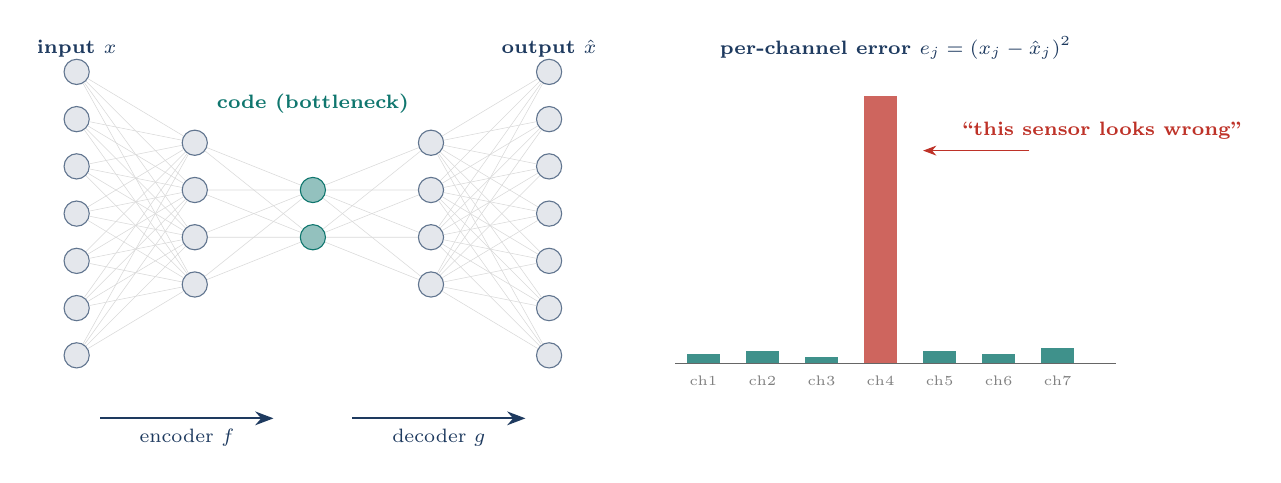
\begin{tikzpicture}[n/.style={circle,draw=mznavy!70,fill=mznavy!12,minimum size=3.2mm,inner sep=0pt},
  c/.style={circle,draw=mzteal,fill=mzteal!45,minimum size=3.2mm,inner sep=0pt}]
\foreach \i in {1,...,7}{\node[n] (a\i) at (0,1.8-0.6*\i+0.6) {}; \node[n] (e\i) at (6,1.8-0.6*\i+0.6) {};}
\foreach \i in {1,...,4}{\node[n] (b\i) at (1.5,1.2-0.6*\i+0.3) {}; \node[n] (d\i) at (4.5,1.2-0.6*\i+0.3) {};}
\foreach \i in {1,2}{\node[c] (c\i) at (3,0.6-0.6*\i+0.3) {};}
\begin{scope}[on background layer/.style={},black!15,very thin]
\foreach \i in {1,...,7}{\foreach \j in {1,...,4}{\draw (a\i)--(b\j); \draw (d\j)--(e\i);}}
\foreach \i in {1,...,4}{\foreach \j in {1,2}{\draw (b\i)--(c\j); \draw (c\j)--(d\i);}}
\end{scope}
\node[font=\scriptsize\bfseries,text=mznavy] at (0,2.1) {input $x$};
\node[font=\scriptsize\bfseries,text=mznavy] at (6,2.1) {output $\hat x$};
\node[font=\scriptsize\bfseries,text=mzteal] at (3,1.4) {code (bottleneck)};
\draw[mznavy,thick,-{Stealth}] (0.3,-2.6)--(2.5,-2.6) node[midway,below,font=\scriptsize] {encoder $f$};
\draw[mznavy,thick,-{Stealth}] (3.5,-2.6)--(5.7,-2.6) node[midway,below,font=\scriptsize] {decoder $g$};
% per-channel error bars (illustrative values)
\begin{scope}[xshift=7.6cm,yshift=-1.9cm]
\node[font=\scriptsize\bfseries,text=mznavy] at (2.8,4.0) {per-channel error $e_j=(x_j-\hat x_j)^2$};
\draw[black!60] (0,0)--(5.6,0);
\foreach \k/\h in {1/0.12,2/0.15,3/0.08,4/3.4,5/0.15,6/0.12,7/0.19}{
  \ifnum\k=4 \fill[mzred!75] (\k*0.75-0.6,0) rectangle ++(0.42,\h);
  \else \fill[mzteal!80] (\k*0.75-0.6,0) rectangle ++(0.42,\h); \fi
  \node[font=\tiny,text=black!50] at (\k*0.75-0.39,-0.22) {ch\k};}
\draw[mzred,-{Stealth}] (4.5,2.7)--(3.15,2.7);
\node[font=\scriptsize\bfseries,text=mzred,anchor=west] at (3.5,2.95) {``this sensor looks wrong''};
\end{scope}
\end{tikzpicture}
\caption{Autoencoder principle (left) and the per-channel reconstruction error that localises the faulty
sensor (right; illustrative values).}
\label{g1-fig:ae}
\end{figure}

\paragraph{Role in our design.} Trained on clean windows only; captures correlated-sensor inconsistencies and
subtle waveform changes that thresholds miss, and gives channel-level evidence for the explanation sentence
(``channel 4 deviates most'').

\subsubsection{The Methods at a Glance}
\begin{table}[H]
\centering
\caption{Qualitative comparison, our assessment from the cited literature~\cite{chandola,pang} and the
experiment in Section~\ref{g1-sec:experiment}. Green = favourable, amber = acceptable, red = costly.}
\label{g1-tab:glance}
\small
\renewcommand{\arraystretch}{1.15}
\begin{tabularx}{\textwidth}{@{}>{\raggedright\arraybackslash}p{2.3cm}>{\raggedright\arraybackslash}p{1.2cm}>{\raggedright\arraybackslash}p{1.8cm}>{\raggedright\arraybackslash}p{2.2cm}LL@{}}
\toprule\hdr
\textbf{Method} & \textbf{Labels} & \textbf{Run cost} & \textbf{Explainable} & \textbf{Strong on} & \textbf{Weak on} \\
\midrule
Rules / physics & \cellcolor{good}none & \cellcolor{good}very low & \cellcolor{good}by design & Impossible values, data-only injection, voltage offset & Bias and bypass (physics still holds) \\
Robust $z$ / CUSUM & \cellcolor{good}none & \cellcolor{good}very low & \cellcolor{good}high & Spikes; persistent offsets & Seasonal baselines (feeder balance) \\
Isolation Forest & \cellcolor{good}none & \cellcolor{good}low & \cellcolor{fair}medium (TreeSHAP) & Global outliers, many features & Shifts inside the normal range \\
One-Class SVM & \cellcolor{good}none & \cellcolor{poor}high on big data & \cellcolor{poor}low (post-hoc) & Smooth boundary on compact data & Scale; kernel tuning \\
Autoencoder & \cellcolor{good}none & \cellcolor{fair}medium (training) & \cellcolor{fair}medium (per channel) & Correlated-sensor, waveform change & Can reconstruct anomalies too well \\
\bottomrule
\end{tabularx}

\end{table}

% =====================================================================
\subsection{Putting It Together: Our Hybrid Detection Stack}
\label{g1-sec:stack}

\begin{figure}[H]
\centering
\resizebox{\textwidth}{!}{%
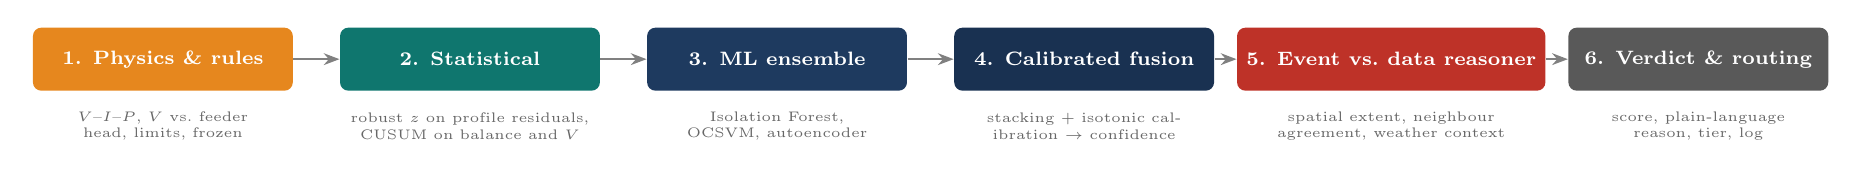
\begin{tikzpicture}[
  st/.style={rounded corners=3pt,text=white,font=\scriptsize\bfseries,minimum width=33mm,minimum height=8mm,align=center},
  sub/.style={font=\tiny,text=black!60,align=center,text width=32mm},
  >={Stealth[length=2mm]}]
\foreach \i/\name/\col/\txt in {
  1/1. Physics \& rules/mzorange/{$V$--$I$--$P$, $V$ vs.\ feeder head, limits, frozen},
  2/2. Statistical/mzteal/{robust $z$ on profile residuals, CUSUM on balance and $V$},
  3/3. ML ensemble/mznavy/{Isolation Forest,\\ OCSVM, autoencoder},
  4/4. Calibrated fusion/mznavy!85!black/{stacking + isotonic calibration $\rightarrow$ confidence},
  5/5. Event vs.\ data reasoner/mzred/{spatial extent, neighbour agreement, weather context},
  6/6. Verdict \& routing/black!65/{score, plain-language reason, tier, log}}{
  \node[st,fill=\col] (s\i) at (\i*3.9,0) {\name};
  \node[sub] at (\i*3.9,-0.85) {\txt};}
\foreach \a/\b in {1/2,2/3,3/4,4/5,5/6}{\draw[->,black!50,thick] (s\a)--(s\b);}
\end{tikzpicture}}
\caption{The detection pipeline. Rules can veto or force escalation; ML scores add sensitivity; the
reasoner decides \emph{what kind} of unusual it is.}
\label{g1-fig:stack}
\end{figure}

\paragraph{How the verdict is reached.} Layers 1--3 answer ``is something unusual?'' and are \emph{meant} to
fire on genuine events too; layer 5 answers ``what kind?'' from consistency features
(Table~\ref{g1-tab:reasoner}). Layers 5--6 are specified in Sections~\ref{g2-sec:goal2} and~\ref{g3-sec:goal3}; this section covers layers 1--4.

\begin{table}[H]
\centering
\caption{Consistency features used by the event-versus-data reasoner.}
\label{g1-tab:reasoner}
\small
\begin{tabularx}{0.85\textwidth}{@{}>{\raggedright\arraybackslash}p{5cm}LL@{}}
\toprule\hdr
\textbf{Evidence} & \textbf{Genuine event} & \textbf{Data-quality problem} \\
\midrule
Spatial extent (meters affected) & Many & One or a few \\
Physical consistency ($V$, $I$, $P$) & Holds & Violated (data-only injection) or holds (bias, bypass) \\
Feeder energy balance & Unchanged & Opens (under-reporting) or goes negative (inflation) \\
Supply & $V=0$ on many meters (outage) & $V>0$ \\
Agreement with correlated neighbours & Yes & Contradicts them \\
Temporal shape & Physical dynamics & Step, frozen, replayed \\
Weather / time-of-day context & Explains it & Does not explain it \\
\bottomrule
\end{tabularx}

\end{table}

\subsubsection{Results on Node N1 of the Challenge Dataset}
\label{g1-sec:experiment}
\paragraph{Set-up.} Unit of analysis: one meter-day (48 readings) of node N1, from 8~January (the profiles need
one week of history) to 31~December, excluding days that are mostly missing: \nOneDays{} meter-days, of which
\nOneClean{} are clean and the rest belong to \nOneEvents{} labelled events. Every detector is trained on clean
meter-days only; labels are used only to score. Thresholds give a 1\% false-positive rate on held-out clean
days (the stack: rules, or any learned detector at 0.25\%). Everything is out-of-fold over 5~folds, with clean
days grouped by meter-week and anomalous days grouped by event, so no event is split. A time split is not
possible: in N1, November--December contain no falsification and no sensor-bias event. An event counts as
\emph{detected} when at least 20\% of its meter-days are flagged (any flag for events of five days or less),
so a long event is not ``caught'' by a chance alarm. Code: \texttt{n1\_experiment.py}.

\begin{table}[H]
\centering
\caption{Node N1, out-of-fold. ``days'': share (\%) of the class's meter-days flagged (darker = higher).
``events'': events detected / events. False positives: share of clean meter-days flagged. Genuine events:
outage, load shedding, sag, swell, surge, cable fault, transformer; meter faults: corruption and sensor faults;
falsification: the 8 manipulation types. Simulated data.}
\label{g1-tab:experiment}
\small
\setlength{\tabcolsep}{4pt}
\begin{tabular}{@{}l cc cc cc |c@{}}
\toprule\hdr
 & \multicolumn{2}{c}{\textbf{Genuine event}} & \multicolumn{2}{c}{\textbf{Meter fault}} & \multicolumn{2}{c|}{\textbf{Falsification}} & \textbf{False} \\
\hdr\textbf{Detector} & days & events & days & events & days & events & \textbf{positives} \\
\midrule
% generated by n1_experiment.py
Rules (layer 1) & \hc{42} & 17/36 & \hc{29} & 18/30 & \hc{66} & 5/8 & 0.0\% \\
Robust z & \hc{1} & 3/36 & \hc{26} & 12/30 & \hc{61} & 5/8 & 1.1\% \\
CUSUM & \hc{1} & 4/36 & \hc{12} & 2/30 & \hc{6} & 0/8 & 2.1\% \\
Isolation Forest & \hc{3} & 11/36 & \hc{7} & 15/30 & \hc{9} & 2/8 & 0.9\% \\
One-Class SVM & \hc{74} & 30/36 & \hc{31} & 25/30 & \hc{67} & 6/8 & 1.3\% \\
Autoencoder & \hc{74} & 30/36 & \hc{28} & 22/30 & \hc{64} & 5/8 & 1.1\% \\
Detection stack & \hc{74} & 30/36 & \hc{31} & 23/30 & \hc{69} & 6/8 & 2.3\% \\
\bottomrule
% ends with \bottomrule
\end{tabular}

\end{table}

\begin{table}[H]
\centering
\caption{The \nRare{} falsification and sensor-fault events of N1, one by one (most types occur once, so
percentages per type would be meaningless). R = rules, z = robust $z$, C = CUSUM, IF, SVM, AE = autoencoder.
First flag and days flagged refer to the whole stack. Balance alarm: first day the CUSUM on the feeder's daily
energy-balance gap fires (it is in alarm on \balFPR\% of clean feeder-days); it names a feeder, not a meter.}
\label{g1-tab:events}
\small
\setlength{\tabcolsep}{4pt}
\resizebox{\textwidth}{!}{%
\begin{tabular}{@{}l c c r l l r l@{}}
\toprule\hdr
\textbf{Event (N1)} & \textbf{Feeder} & \textbf{Start} & \textbf{Days} & \textbf{Detected by} & \textbf{First flag} & \textbf{Days flagged} & \textbf{Balance alarm} \\
\midrule
% generated by n1_experiment.py
\texttt{partial\_reduction\_bypass} & F2 & 04 Feb & 60 & -- & day 8 & 18\% & day 13 \\
\texttt{selective\_bypass} & F2 & 09 Feb & 65 & -- & day 3 & 5\% & day 8 \\
\texttt{meter\_zeroing} & F1 & 11 May & 20 & IF, SVM & day 0 & 22\% & -- \\
\texttt{fdi\_scale} & F3 & 02 May & 63 & R, z, SVM, AE & day 1 & 98\% & day 14 \\
\texttt{fdi\_evasion} & F2 & 25 Apr & 35 & R, z, IF, SVM, AE & day 0 & 100\% & day 9 \\
\texttt{fdi\_inflate} & F3 & 12 Sep & 33 & R, z, SVM, AE & day 1 & 97\% & day 13 \\
\texttt{fdi\_replay} & F2 & 09 Aug & 29 & R, z, SVM, AE & day 0 & 100\% & -- \\
\texttt{coordinated\_fdi} & F1 & 14 Oct & 26 & R, z, SVM, AE & day 0 & 100\% & day 6 \\
\texttt{bias\_step} & F1 & 05 Jun & 58 & -- & day 2 & 5\% & day 14 \\
\texttt{gain\_drift} & F2 & 19 Apr & 66 & -- & -- & 0\% & day 15 \\
\texttt{gain\_drift} & F2 & 18 May & 65 & -- & day 42 & 2\% & day 16 \\
\texttt{clock\_shift} & F1 & 23 Feb & 15 & -- & -- & 0\% & -- \\
\texttt{voltage\_offset\_drift} & F1 & 10 Apr & 64 & R, z, C, SVM, AE & day 0 & 100\% & day 3 \\
\texttt{stuck\_value} & F1 & 12 Feb & 3 & R, z, IF, SVM, AE & day 0 & 100\% & -- \\
\texttt{stuck\_value} & F2 & 28 Jun & 1 & R, z, IF, SVM, AE & day 0 & 100\% & -- \\
\texttt{stuck\_value} & F3 & 10 Nov & 2 & -- & -- & 0\% & -- \\
\bottomrule
% ends with \bottomrule
\end{tabular}}

\end{table}

\needspace{8\baselineskip}
\paragraph{What the results show.}
\begin{itemize}[leftmargin=*,itemsep=2pt]
  \item \textbf{The stack is usable as a first filter.} It flags \stackFPR\% of clean meter-days. The physics
        and domain rules alone flag none, yet they catch every data-only injection, the voltage offset and two of
        the three stuck meters from the first or second day (the third froze for 4~hours across midnight,
        below the 3-hour-per-day limit on either side).
  \item \textbf{No detector wins everywhere.} The One-Class SVM and the autoencoder carry the learned part
        (about three quarters of genuine-event days, most meter-fault events). Robust $z$ is strong on
        falsification days but blind to genuine events. Isolation Forest is weak at this false-positive rate:
        most anomalies here shift values \emph{inside} the normal range rather than isolate them.
  \item \textbf{The hard cases are the physically consistent ones.} Partial and selective bypass, the
        constant bias and both gain drifts keep $V$, $I$ and $E$ consistent and are flagged on at most 18\% of
        their days, as is a clock shift. This matches the difficulty ranking we gave in the data card.
  \item \textbf{The feeder balance sees them, but only as a feeder.} Its CUSUM fires 8--16 days after the start
        of both bypasses, the bias and both drifts. Pointing to the right meter fails: a household's daily
        share of its feeder varies far more than a 7--14\% bias, and the gap itself moves: about \gapSd{}~points of
        day-to-day noise on clean days, plus a spring--summer drop when PV homes export. Phase~2 will model
        the expected gap from feeder load, PV export and temperature, run CUSUM on the residual, and attribute
        alarms with longer windows.
  \item \textbf{Limits.} Simulated data from one generator; most falsification and sensor types occur once in
        N1, so these are case results, not rates. Feeder-level references use clean feeder-days.
\end{itemize}

\subsubsection{Output to the Explanation Layer (Goal 2)}
For every flagged meter-day, the detection layer passes on: the stack decision and each detector's score; which rules
fired, with the measured value and threshold; the neighbourhood support (share of the feeder's 10 meters flagged
the same day); the feeder-balance alarm state; and the autoencoder's per-feature reconstruction error, which
tells Goal~2 which channel looks wrong.


\clearpage
% generated by build_parts.py from the goal report -- edit the report, not this file
% ===================== BEGIN GOAL 2 SECTION =====================
\providecommand{\GE}{\texttt{GENUINE\_EVENT}}
\providecommand{\MF}{\texttt{METER\_FAULT}}
\providecommand{\SD}{\texttt{SUSPICIOUS\_DATA}}
\providecommand{\ND}{\texttt{NO\_DATA}}
\providecommand{\NORM}{\texttt{NORMAL}}

\section{Goal 2: Confidence Scores and Explainability}
\label{g2-sec:goal2}

\subsection{Goal and Requirements}
The challenge requires that every flagged event comes with a verdict that a human can understand and
verify. The system must output a confidence score, provide a plain-language explanation, and maintain an
auditable decision log that records what was detected, concluded and why. It should use interpretable
approaches and avoid black-box scoring whose reasoning cannot be examined.

Anomalies in this project are equipment and measurement problems, suspected data manipulation (theft or
false data injection) and genuine electrical events. The component therefore chooses among four verdicts,
the same four that the escalation layer of Goal~3 routes: \NORM, \GE{} (the data is right and the grid did
something), \MF{} (a faulty or corrupted meter) and \SD{} (readings that look manipulated). A fifth outcome,
\ND, records a communication loss, which is not scored. The prototype runs on node N1 of the EnergyMind
dataset: one transformer, 30 smart meters on three feeders of 10, readings every 30~minutes.
Table~\ref{g2-tab:requirements} maps each requirement to a design element of this section.

\begin{table}[H]
\centering
\caption{Requirements of Challenge Goal 2 and where this design meets them.}
\label{g2-tab:requirements}
\small
\begin{tabularx}{\textwidth}{@{}>{\raggedright\arraybackslash}p{3.4cm}LL@{}}
\toprule\hdr
\textbf{Requirement} & \textbf{Design element} & \textbf{Artifact produced} \\
\midrule
Confidence score & Calibrated probability of each of the four verdicts, obtained by multinomial Platt scaling of a few inspectable inputs (Section~\ref{g2-sec:confidence}) & Fields \texttt{class\_probabilities}, \texttt{confidence}, \texttt{band}; calibration curve, Brier score \\ \addlinespace
Plain-language explanation & Rules + SHAP $\rightarrow$ evidence $\rightarrow$ structured summary $\rightarrow$ LLM text (no retrieval), checked against the rule trace, the SHAP ranking and the logged evidence before it is shown (Section~\ref{g2-sec:language}) & Verdict card; field \texttt{llm\_diagnosis} with the result of the faithfulness check \\ \addlinespace
Auditable decision log & One hash-chained record per flagged meter-day (Section~\ref{g2-sec:log}) & \texttt{decision\_log.jsonl} \\ \addlinespace
Record what was detected, concluded and why & Three explicit blocks in every record: \texttt{detected}, \texttt{concluded}, \texttt{why} & Rule trace, SHAP evidence, neighborhood support \\ \addlinespace
Interpretable approaches & Rule-backed verdicts; SHAP on the detector scores; a calibration model whose coefficients can be printed & No verdict whose reasoning cannot be inspected \\
\bottomrule
\end{tabularx}

\end{table}

\subsection{Inputs and Outputs of this Component}
\label{g2-sec:io}
The detection layer of Goal~1 works on \emph{meter-days} (48 readings of one meter) and, for every flagged
meter-day, passes on: the stack decision and each detector's score (rules, robust $z$, CUSUM, Isolation
Forest, One-Class SVM, autoencoder); which rules fired, with the measured value and threshold; the
neighborhood support (share of the other 9 meters of the feeder flagged the same day); the state of the
feeder energy-balance alarm; and the autoencoder's per-feature reconstruction error. This component adds a
few evidence quantities computed from the same day's readings (Section~\ref{g2-sec:evidence}) and produces, for
every flagged meter-day, a verdict with its sub-type, the four class probabilities and a confidence band, the
supporting evidence, a plain-language explanation and one decision-log record. The class probabilities are
the input of the Goal~3 escalation layer.

\subsection{Design Principles}
\begin{enumerate}[leftmargin=*,itemsep=2pt]
  \item \textbf{The LLM only describes.} The language model never detects an anomaly and never changes a verdict or a confidence value. This follows the conclusion of the rule-aware prompting work that the main value of an LLM here is a readable rationale for the operator rather than a replacement for the detector~\cite{ruleaware}.
  \item \textbf{Every statement is traceable.} Each statement in an explanation points to a logged item: a rule that fired, a feature value, or a SHAP contribution.
  \item \textbf{Confidence is measured.} The score is calibrated on labeled events and its quality is evaluated like any other output of the system (Section~\ref{g2-sec:evaluation}).
  \item \textbf{No explanation without evidence.} If the generated text fails the faithfulness check, the structured summary is shown instead.
\end{enumerate}

\subsection{Evidence Available to the Explanation Layer}
\label{g2-sec:evidence}
We index a flagged meter-day by meter $i$ and day $t$. Goal~1 supplies the detector scores, the fired rules
and the neighborhood support $s_{i,t}$; the neighborhood-support idea follows prior work that adjusts an
anomaly score using temporal context and the neighborhood~\cite{multiuser}. This component computes the
evidence vector $\mathbf{e}_{i,t}$ of Table~\ref{g2-tab:evidence} from the meter's 48 readings. We write $E$ for
the energy imported in a 30-minute interval ($\Delta t=0.5$~h), $V$, $I$ and $\mathrm{PF}$ for voltage,
current and power factor, $V^{\mathrm{head}}$ for the voltage measured at the head of the feeder and $X$ for
the exported PV energy. Baselines (profiles, medians, scales) are learned on clean meter-days only, i.e.\ days
whose 48 readings are all labelled normal.

\begin{table}[H]
\centering
\caption{Evidence vector $\mathbf{e}_{i,t}$ of a flagged meter-day.}
\label{g2-tab:evidence}
\small
\begin{tabularx}{\textwidth}{@{}>{\raggedright\arraybackslash}p{1.3cm}>{\raggedright\arraybackslash}p{6.2cm}L@{}}
\toprule\hdr
\textbf{Symbol} & \textbf{Definition} & \textbf{What it tells a human} \\
\midrule
$v^{0}_{i,t}$ & Share of readings with $V=0$, or a \texttt{power\_fail} entry in the meter's event log & Supply was lost: the meter is reporting a real outage \\ \addlinespace
$g_{i,t}$ & Share of missing readings & Communication loss \\ \addlinespace
$\phi_{i,t}$ & Longest run of readings in which energy \emph{and} voltage are both unchanged (only while $V>0$ and $X=0$) & A stuck meter freezes every channel; real voltage never repeats for hours \\ \addlinespace
$\rho_{i,t}$ & Median over the day of $E\,/\,(V I\,\mathrm{PF}\,\Delta t/1000)$, using only readings with $V>0$, $X=0$ and an expected energy above 0.02~kWh & Electrical consistency: 1 when energy, voltage and current agree; skipped while the home exports PV \\ \addlinespace
$s_{i,t}$ & Share of the other 9 meters of the feeder flagged the same day (from Goal~1) & One house, part of the feeder, or the whole feeder \\ \addlinespace
$\Delta V_{i,t}$ & 24-h median of $V-V^{\mathrm{head}}$ & A meter cannot read more than its feeder head: a positive excess is a voltage-sensor offset \\ \addlinespace
$\delta_{i,t}$ & Relative drop of the day's energy below the meter's own 28-day profile & How much less than usual this home reports \\ \addlinespace
$b_{i,t}$ & Feeder energy-balance alarm (from Goal~1): on when the feeder's daily loss has moved away from its seasonal reference & Energy is disappearing (or appearing) somewhere on this feeder \\ \addlinespace
$\kappa^{\mathrm{tamp}}_{i,t}$ & \texttt{magnetic\_tamper} or \texttt{cover\_open} in the meter's event log & Weak hint of physical tampering (the log also has false alarms) \\ \addlinespace
$c^{\mathrm{drift}}_{i,t}$ & CUSUM alarm of Goal~1 on the meter's voltage offset, or slope of the meter's share of the feeder over 14 days & Slow drift or a persistent offset \\ \addlinespace
$\pi_{i,t}$ & Number of consecutive flagged days for this meter while its neighbors are not flagged & How long the deviation has lasted \\
\bottomrule
\end{tabularx}

\end{table}

\paragraph{Why these quantities, on this dataset.} Three facts of node N1 shaped the list.
(i) A supply loss is recorded as zeros, not as missing data: in N1 the 683 supply-loss readings of outages, load
shedding, cable faults and the transformer trip have $V=0$, while only communication losses are blank. Without
$v^{0}$ a flat zero would look like a frozen meter. (ii) The consistency $\rho$ is meaningful because the
dataset's \emph{data-only} injections edit the energy field alone ($\rho\approx0.65$--$0.69$, or $1.68$ for
inflated readings), while honest meters already carry about 1\% measurement error. Without the export gate,
$\rho$ would fire on 39\% of the clean readings of N1's three PV homes; with it, on 0.25\% of all clean
readings. (iii) Sensor bias and physical bypass scale energy \emph{and} current together, so $\rho$ stays at 1
for them; what reveals a bypass is a large drop $\delta$ against the meter's own history together with the
feeder balance $b$.

\subsection{Rule-Backed Verdict Layer}
\label{g2-sec:rules}
The rule-backed scoring turns the evidence vector into a verdict and a sub-type (Figure~\ref{g2-fig:rules}).
Rules are evaluated in a fixed order, so the first matching rule is the one reported, and its identifier
appears in the log and in the explanation. The order follows what makes the other evidence unreliable: a lost
supply first (otherwise a flat zero looks like a frozen meter), then missing and frozen data, then physical
consistency, which separates a manipulated or corrupted value from a real change, and only then the
neighborhood support, which decides between a feeder-wide event and a local one. The split between sudden
problems (R2, R3) and slow ones (R5, R5b) mirrors the split between point and contextual anomalies reported for
smart-meter data~\cite{timefreq}.

\begin{figure}[H]
\centering
\resizebox{\textwidth}{!}{%
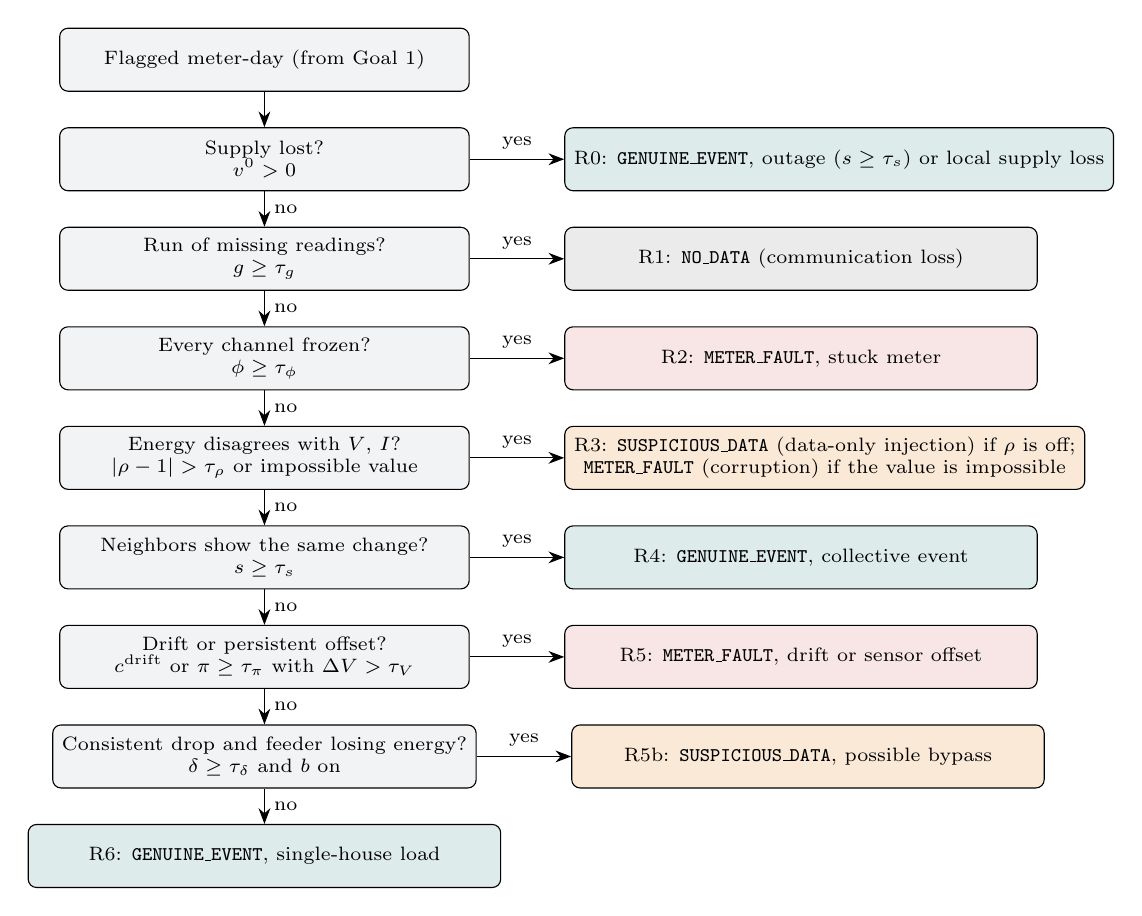
\begin{tikzpicture}[
  node distance=4.5mm and 12mm,
  q/.style={draw,rounded corners=3pt,fill=blue!6,align=center,minimum width=52mm,minimum height=8mm,font=\scriptsize},
  r/.style={draw,rounded corners=3pt,align=center,minimum width=60mm,minimum height=8mm,font=\scriptsize},
  fault/.style={r,fill=red!12}, event/.style={r,fill=green!14}, susp/.style={r,fill=orange!18},
  nodata/.style={r,fill=black!8},
  >={Stealth[length=2mm]}, lab/.style={font=\scriptsize,midway,above}]
\node[q] (s0) {Flagged meter-day (from Goal 1)};
\node[q,below=of s0] (q0) {Supply lost?\\ $v^{0}>0$};
\node[q,below=of q0] (q1) {Run of missing readings?\\ $g\ge\tau_g$};
\node[q,below=of q1] (q2) {Every channel frozen?\\ $\phi\ge\tau_\phi$};
\node[q,below=of q2] (q3) {Energy disagrees with $V$, $I$?\\ $|\rho-1|>\tau_\rho$ or impossible value};
\node[q,below=of q3] (q4) {Neighbors show the same change?\\ $s\ge\tau_s$};
\node[q,below=of q4] (q5) {Drift or persistent offset?\\ $c^{\mathrm{drift}}$ or $\pi\ge\tau_\pi$ with $\Delta V>\tau_V$};
\node[q,below=of q5] (q6) {Consistent drop and feeder losing energy?\\ $\delta\ge\tau_\delta$ and $b$ on};
\node[event,below=of q6] (e2) {R6: \GE{}, single-house load};
\node[event,right=of q0] (r0) {R0: \GE{}, outage ($s\ge\tau_s$) or local supply loss};
\node[nodata,right=of q1] (r1) {R1: \ND{} (communication loss)};
\node[fault,right=of q2] (r2) {R2: \MF{}, stuck meter};
\node[susp,right=of q3] (r3) {R3: \SD{} (data-only injection) if $\rho$ is off;\\ \MF{} (corruption) if the value is impossible};
\node[event,right=of q4] (r4) {R4: \GE{}, collective event};
\node[fault,right=of q5] (r5) {R5: \MF{}, drift or sensor offset};
\node[susp,right=of q6] (r5b) {R5b: \SD{}, possible bypass};
\draw[->] (s0)--(q0);
\foreach \a/\b in {q0/q1,q1/q2,q2/q3,q3/q4,q4/q5,q5/q6,q6/e2}{\draw[->] (\a)--node[right,font=\scriptsize]{no}(\b);}
\foreach \a/\b in {q0/r0,q1/r1,q2/r2,q3/r3,q4/r4,q5/r5,q6/r5b}{\draw[->] (\a)--node[lab]{yes}(\b);}
\end{tikzpicture}}
\caption{Rule cascade turning the evidence vector into a verdict. All thresholds $\tau$ are fitted by
event-grouped cross-validation (Section~\ref{g2-sec:confidence}) and stored in a versioned configuration file
(\texttt{configs/thresholds.yaml}), not hard-coded.}
\label{g2-fig:rules}
\end{figure}

\begin{table}[H]
\centering
\caption{Rule table. The tamper flag $\kappa^{\mathrm{tamp}}$ is reported as supporting evidence for R5b but
never decides a verdict: in N1 it appears on 4 falsified readings and on 55 clean ones.}
\label{g2-tab:rules}
\small
\begin{tabularx}{\textwidth}{@{}>{\raggedright\arraybackslash}p{0.9cm}>{\raggedright\arraybackslash}p{3.7cm}>{\raggedright\arraybackslash}p{3.1cm}L@{}}
\toprule\hdr
\textbf{Rule} & \textbf{Condition} & \textbf{Verdict} & \textbf{Reason sentence (template)} \\
\midrule
R0 & $v^{0}>0$ & \GE{} (outage if $s\ge\tau_s$; local supply loss if 2--6 meters; single meter otherwise) & ``Voltage was 0~V on \{n\} of \{N\} meters of feeder \{f\} for \{hours\} h: supply was lost and the meter is reporting correctly.'' \\ \addlinespace
R1 & $g\ge\tau_g$ & \ND{} (communication loss) & ``\{share\} of this meter's readings did not arrive; no verdict is possible for this period.'' \\ \addlinespace
R2 & $\phi\ge\tau_\phi$ & \MF{} (stuck meter) & ``Energy and voltage have not changed for \{hours\} h; real voltage always varies.'' \\ \addlinespace
R3 & $|\rho-1|>\tau_\rho$ & \SD{} (data-only injection); \MF{} (corruption) if $E<0$, $E=99.999$ or $\times1000$ & ``Reported energy is \{ratio\}$\times$ what voltage and current imply (limit \{tau\}); voltage and current look normal.'' \\ \addlinespace
R4 & $s\ge\tau_s$, $\rho$ consistent & \GE{} (collective) & ``\{n\} of \{N\} meters on feeder \{f\} changed together and their electrical readings agree.'' \\ \addlinespace
R5 & $s<\tau_s$, $c^{\mathrm{drift}}$ on, or $\Delta V>\tau_V$ for $\ge\tau_\pi$ days & \MF{} (drift or sensor offset) & ``This meter reads \{dv\}~V above its feeder head, which is physically impossible, for \{days\} days.'' \\ \addlinespace
R5b & $s<\tau_s$, $\rho$ consistent, $\delta\ge\tau_\delta$, $b$ on & \SD{} (possible bypass) & ``This home reports \{pct\}\% less than its usual level for \{days\} days while feeder \{f\} loses \{gap\}\% more energy than usual; voltage and current agree with the reported energy, which fits a physical bypass.'' \\ \addlinespace
R6 & $s<\tau_s$, $\rho$ consistent, short-lived & \GE{} (single-house load) & ``Only this home changed, briefly, and energy, voltage and current agree: an appliance switching on is the likely cause.'' \\
\bottomrule
\end{tabularx}

\end{table}

\paragraph{Notes on the rules.}
\begin{itemize}[leftmargin=*,itemsep=2pt]
  \item \textbf{R0 before R2.} Without it, every outage, load-shedding period, cable fault and transformer trip
        of N1 would be reported as a stuck meter, the opposite of the right answer.
  \item \textbf{R3 before R4.} A coordinated injection hits three meters of one feeder, so it could pass the
        neighborhood test; its energy disagrees with $V$ and $I$, so R3 catches it first.
  \item \textbf{Suspect channel.} For R3 the suspect channel is energy by construction. For the other
        verdicts it is the feature with the largest autoencoder reconstruction error passed on by Goal~1; for
        faults that scale every channel (bias, bypass, frozen meter, clock shift) no single channel is
        named.
  \item \textbf{R5b before R6.} An isolated, electrically consistent drop is not automatically an appliance:
        when it lasts and the feeder starts losing energy at the same time, a bypass is the better
        explanation. A short, isolated, consistent change with no balance alarm stays a single-house load.
  \item \textbf{What the rules cannot settle.} Goal~1 found that small sensor biases and gain drifts are
        rarely flagged at all, and that the balance alarm names a feeder, not a meter. When $b$ is on but no
        meter shows a clear drop, the case is logged as \SD{} with a low confidence band, which sends it to
        a human (Goal~3).
\end{itemize}

\subsection{Confidence Score}
\label{g2-sec:confidence}
For each flagged meter-day the component outputs a probability for each of the four verdicts,
$p_{i,t}(c)$ for $c\in\{\NORM,\GE,\MF,\SD\}$. The confidence of the reported verdict is
$c_{i,t}=p_{i,t}(\hat c)$, and the full vector is passed to Goal~3, which needs the margin between the two most
likely verdicts and the set of plausible alternatives. The probabilities are built from three inputs, each
of which can be inspected on its own:
\begin{enumerate}[leftmargin=*,itemsep=2pt]
  \item the Goal~1 stack score $\tilde a_{i,t}$: the largest detector score, each standardized against its
        distribution on clean meter-days;
  \item the \emph{rule margin} $m_{i,t}\in[0,1]$, which measures how clearly the rule that fired was
      satisfied. Each condition of that rule compares an evidence value $e_j$ with a threshold $\tau_j$.
      For each condition we compute its relative distance from the threshold,
      $\min\{1,\,|e_j-\tau_j|/\tau_j\}$, which is $0$ when the value sits exactly on the threshold and
      $1$ when it is at least one threshold-width away. The margin $m_{i,t}$ is the smallest of these
      values over the conditions of the rule, so a verdict is only as clear as its most borderline
      condition;
  \item the \emph{detector agreement} $\kappa_{i,t}\in\{0,\dots,6\}$: how many of the six Goal~1 detectors
        flagged the day, in the spirit of the explicit sigma rule used in rule-aware
        prompting~\cite{ruleaware}.
\end{enumerate}
Together with a one-hot code of the rule that fired, these inputs are mapped to probabilities by multinomial
Platt scaling, one of the calibration techniques listed in the trust-calibration literature~\cite{trustcal}:
a multinomial logistic regression whose coefficients can be printed and read,
\begin{equation}
  p_{i,t}(c)\;=\;\frac{\exp\bigl(\beta_{c,0}+\beta_{c,1}\tilde a_{i,t}+\beta_{c,2}m_{i,t}+\beta_{c,3}\kappa_{i,t}+\gamma_{c,r(i,t)}\bigr)}
  {\sum_{c'}\exp\bigl(\beta_{c',0}+\beta_{c',1}\tilde a_{i,t}+\beta_{c',2}m_{i,t}+\beta_{c',3}\kappa_{i,t}+\gamma_{c',r(i,t)}\bigr)},
\end{equation}
where $r(i,t)$ is the rule that fired. The target is the true class of the meter-day, known from the dataset
labels. If the calibration curve is poor, isotonic regression, another technique from the same
literature~\cite{trustcal}, is the alternative.

\paragraph{Confidence band.} The probability is shown to operators as a band: HIGH above 0.90, LOW below
0.60, MEDIUM in between (Goal~3 thresholds). A class's band may be HIGH only if its calibration has been
validated on at least 30 out-of-fold events. In N1 this holds for \GE{} (37 events) and \MF{} (33), not for
\SD{} (8 events, one per manipulation type), so \SD{} verdicts are capped at MEDIUM and are always reviewed by
a human.

We do not assume that the result is calibrated; we measure it (Section~\ref{g2-sec:evaluation}). This matters because the confidence-based routing of Goal~3 assumes reasonably calibrated confidence: an overconfident model may delegate dangerous decisions to the AI, and an underconfident one may defer everything to humans~\cite{trustcal}.

\paragraph{Data used for fitting.} A split by calendar period does not work on this dataset: in N1,
November--December contain no falsification and no sensor-bias event, and September--October only two
falsifications. Baselines (profiles, medians, scales) therefore use clean meter-days only, and the thresholds
$\tau$ and the coefficients $\beta,\gamma$ are fitted by 5-fold cross-validation over the whole year, with folds
grouped by event (\texttt{gt\_event\_id}), so that no event is split between fitting and testing; within each
training fold, $\tau$ is fitted on one half of the events and $\beta,\gamma$ on the other. Clean days are
assigned to folds in meter-week blocks to keep near-duplicate neighboring readings from leaking between sets.
All reported numbers are out-of-fold, per event, with Wilson 95\% intervals.

\subsection{From Evidence to Plain Language}
\label{g2-sec:language}
Figure~\ref{g2-fig:pipeline} shows how the verdict and the evidence become the text that the operator reads,
following the chain rules and SHAP $\rightarrow$ evidence $\rightarrow$ structured summary $\rightarrow$ LLM text.
There is no retrieval step (see ``Why no retrieval'' below). Full explanations are generated only for flagged
meter-days, never for every normal reading, to keep latency and cost down.

\begin{figure}[htbp]
\centering
\resizebox{\textwidth}{!}{%
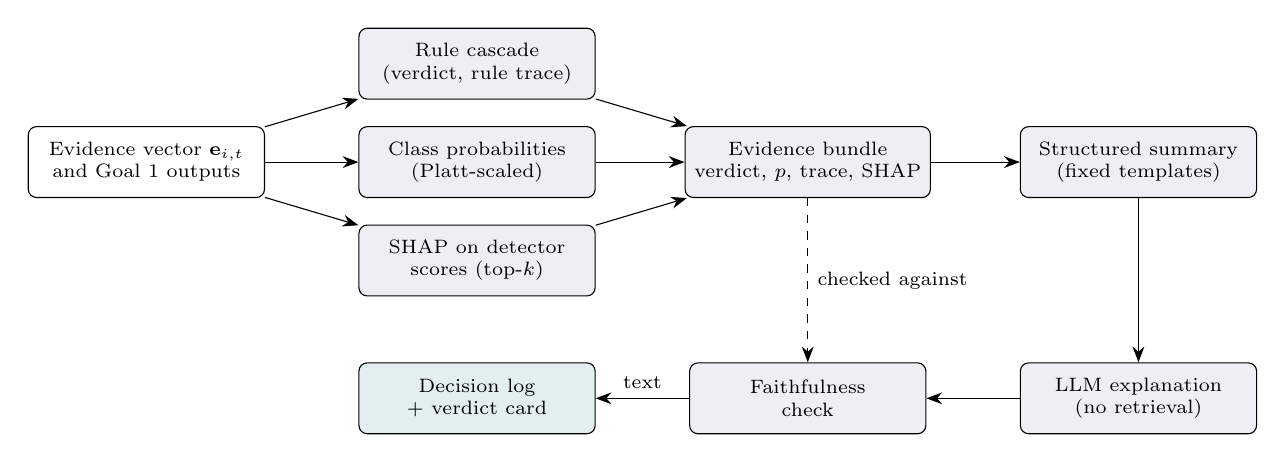
\begin{tikzpicture}[
  b/.style={draw,rounded corners=3pt,align=center,minimum width=30mm,minimum height=9mm,font=\scriptsize},
  core/.style={b,fill=blue!8}, result/.style={b,fill=green!12},
  >={Stealth[length=2mm]}]
\node[b] (ev) at (0,0) {Evidence vector $\mathbf{e}_{i,t}$\\ and Goal 1 outputs};
\node[core] (rules) at (4.2,1.25) {Rule cascade\\ (verdict, rule trace)};
\node[core] (cal) at (4.2,0) {Class probabilities\\ (Platt-scaled)};
\node[core] (shap) at (4.2,-1.25) {SHAP on detector\\ scores (top-$k$)};
\node[core] (bundle) at (8.4,0) {Evidence bundle\\ verdict, $p$, trace, SHAP};
\node[core] (tpl) at (12.6,0) {Structured summary\\ (fixed templates)};
\node[core] (llm) at (12.6,-3.0) {LLM explanation\\ (no retrieval)};
\node[core] (val) at (8.4,-3.0) {Faithfulness\\ check};
\node[result] (log) at (4.2,-3.0) {Decision log\\ + verdict card};
\draw[->] (ev)--(rules); \draw[->] (ev)--(cal); \draw[->] (ev)--(shap);
\draw[->] (rules)--(bundle); \draw[->] (cal)--(bundle); \draw[->] (shap)--(bundle);
\draw[->] (bundle)--(tpl);
\draw[->] (tpl)--(llm);
\draw[->] (llm)--(val);
\draw[->,dashed] (bundle)--node[right,font=\scriptsize]{checked against}(val);
\draw[->] (val)--node[above,font=\scriptsize]{text}(log);
\end{tikzpicture}}
\caption{Explanation pipeline. The language model only rewrites the structured summary; it receives no
retrieved documents, and its text is shown only if it passes the faithfulness check.}
\label{g2-fig:pipeline}
\end{figure}

The language model receives only the evidence bundle and the structured summary, and writes about them; the
faithfulness check compares its text with the same bundle. If the check rejects the text, the structured
summary is logged and shown instead.

\subsubsection*{Step 1: attributions with SHAP}
The rules say what kind of problem it is; SHAP says why the detectors flagged the meter-day in the first
place. SHAP assigns each input feature a value showing how much it pushed a detector's score for this day up
or down relative to a baseline, and it is model-agnostic. We apply the \texttt{shap} library to the Isolation
Forest and the autoencoder of Goal~1, on their daily features, and only on flagged meter-days. Each feature
is tied to a sentence template by a small lexicon, which is how a number becomes a statement
(Table~\ref{g2-tab:lexicon}).

\begin{table}[H]
\centering
\caption{Excerpt of the feature lexicon that turns attributions into sentences (one entry per Goal~1
feature; the evidence quantities of Table~\ref{g2-tab:evidence} have their own sentences in
Table~\ref{g2-tab:rules}).}
\label{g2-tab:lexicon}
\small
\begin{tabularx}{\textwidth}{@{}>{\raggedright\arraybackslash}p{3.6cm}L@{}}
\toprule\hdr
\textbf{Goal 1 feature} & \textbf{Sentence template} \\
\midrule
Profile residual & ``Today this home used \{x\} kWh against a usual \{y\} kWh for this season and day type.'' \\ \addlinespace
Share of the feeder & ``This home's share of feeder \{f\} has moved by \{pct\}\% compared with the last four weeks.'' \\ \addlinespace
Physics ratio & ``Reported energy is \{ratio\}$\times$ what voltage and current imply.'' \\ \addlinespace
$V$ minus feeder-head $V$ & ``This meter reads \{dv\}~V \{above/below\} the head of its feeder; usually \{dv0\}~V.'' \\ \addlinespace
Longest frozen run & ``Energy and voltage stayed identical for \{hours\} h.'' \\ \addlinespace
Lag gain against profile & ``Today's pattern matches the usual one best when shifted by \{h\} h (clock problem?).'' \\ \addlinespace
Similarity to last week & ``Today's readings are almost identical to the same day last week (possible replay).'' \\
\bottomrule
\end{tabularx}

\end{table}

\subsubsection*{Step 2: structured evidence summary}
A deterministic step assembles the evidence bundle into a summary: a headline (verdict, channel, confidence
and band), the strongest reasons (the rule's reason sentence first, then the highest SHAP contributions), the
runner-up verdict, a \emph{what would change this verdict} line generated from the rule thresholds, and a
suggested check. This follows the recommendation, in a review of AI approaches for smart-grid reliability, to
combine local feature attribution, counterfactuals and logged explanations~\cite{review2025}. Every sentence
comes from a template of Table~\ref{g2-tab:rules} or Table~\ref{g2-tab:lexicon}, filled with values from the log. The
summary is the input of the language model and also the text shown if the faithfulness check fails. An
illustrative card (modelled on the data-only injection of feeder N1-F3 in May; values for illustration):

\begin{lstlisting}
Event N1-2025-05-03-M026 | Meter N1-M026 (feeder N1-F3) | 2025-05-03
VERDICT: SUSPICIOUS DATA, energy channel     CONFIDENCE: 0.74 (MEDIUM)
Runner-up: METER FAULT (0.19)

Why:
 1. Reported energy is 0.65x what voltage and current imply
    (limit +/-5%) -> rule R3.
 2. Isolated: 0 of 9 other meters on feeder N1-F3 changed.
 3. Voltage and current follow this home's usual pattern; only the
    energy field is low.

This would be a METER FAULT instead if: the value were impossible
(negative, x1000, 99.999); a GENUINE EVENT if >= 3 neighbors changed
the same way and energy matched voltage and current.

Suggested check: read the meter register on site and compare it with
the reported energy; inspect the data path (gateway, head-end).
\end{lstlisting}

\subsubsection*{Step 3: LLM explanation with a faithfulness check}
The language model turns the structured summary into a readable diagnosis in plain language. It receives the
evidence bundle as structured data and nothing else. It is asked to justify the verdict against an explicit,
stated rule, as in rule-aware prompting for grid telemetry~\cite{ruleaware}, and it may not alter the verdict,
the confidence or the band.

Before the text is displayed, a faithfulness check compares it with the evidence bundle:
\begin{itemize}[leftmargin=*,itemsep=1pt]
  \item every reason it names must be a fired rule or one of the top-$k$ SHAP features;
  \item every number it quotes must match the logged value up to rounding;
  \item the verdict, the confidence and the band must be those in the log.
\end{itemize}
If any test fails, the structured summary is shown instead and the event is logged with that fact. We treat the
LLM as a layer that describes the evidence, not as a source of reasoning.

\paragraph{Why no retrieval (RAG).} We considered giving the language model retrieved context (descriptions of
the fault kinds, the anomaly taxonomy, earlier log entries for the same meter). We dropped it. A study of
retrieval-augmented LLM post-processing for streaming anomaly detection found only a modest gain, and the
faithfulness of the explanations did not improve with retrieval~\cite{ragaudit}. For an operator who must verify
a verdict, that small gain does not justify the extra latency on every flagged case and a document corpus to
build and maintain. Everything the explanation needs is already in the evidence bundle.

\subsection{Auditable Decision Log}
\label{g2-sec:log}
Every flagged meter-day produces one record in an append-only JSON Lines file. Each record stores the hash of
the previous one, so a later edit or deletion breaks the chain. The record is grouped around the three
questions the challenge asks (Table~\ref{g2-tab:log}); an abridged example follows. The escalation layer of
Goal~3 appends its own \texttt{governance} block (route, rules fired, operator judgement, final decision) to the
same record; this section defines only the fields produced by detection, conclusion and explanation. The full
schema is \texttt{docs/decision\_log\_schema.json} in the project repository.

\begin{table}[H]
\centering
\caption{Structure of a decision log record.}
\label{g2-tab:log}
\small
\begin{tabularx}{\textwidth}{@{}>{\raggedright\arraybackslash}p{2.8cm}L@{}}
\toprule\hdr
\textbf{Block} & \textbf{Fields} \\
\midrule
\texttt{detected} & event id, day, node, feeder and meter id, model version, stack score, per-detector scores, per-feature reconstruction error, flag \\ \addlinespace
\texttt{concluded} & verdict, sub-type, suspect channel, class probabilities, confidence, band \\ \addlinespace
\texttt{why} & rule trace (rule id, measured value, threshold, passed or not), SHAP evidence, neighborhood support, feeder-balance alarm, threshold version \\ \addlinespace
\texttt{explanation} & LLM diagnosis, result of the faithfulness check, text actually shown \\ \addlinespace
\texttt{ground\_truth} & filled afterwards, for evaluation only: dataset label, sub-type, event id \\
\bottomrule
\end{tabularx}

\end{table}

\begin{lstlisting}
{"event_id":"N1-2025-05-03-M026","ts":"2025-05-03","node_id":"N1",
 "feeder_id":"N1-F3","meter_id":"N1-M026",
 "detected":{"model_version":"detect-0.1","fused_score":4.8,"flag":true,
   "detector_scores":{"rules":1,"robust_z":9.1,"svm":2.3,"ae":6.4}},
 "concluded":{"verdict":"SUSPICIOUS_DATA","subtype":"data_only_injection",
   "suspect_channel":"energy","confidence":0.74,"band":"MEDIUM",
   "class_probabilities":{"NORMAL":0.02,"GENUINE_EVENT":0.05,
                          "METER_FAULT":0.19,"SUSPICIOUS_DATA":0.74}},
 "why":{"rules":[{"id":"R3","measured":0.65,"threshold":0.05,"passed":true},
                 {"id":"R4","measured":0.0,"threshold":0.3,"passed":false}],
        "shap":[["physics_ratio",0.52],["profile_residual",0.21]],
        "neighbour_support":"0/9","balance_alarm":false,
        "thresholds_version":"0.1-phase1"},
 "explanation":{"llm_diagnosis":"...","faithfulness":"pass","shown":"llm"},
 "prev_hash":"9f2c...","hash":"41ab..."}
\end{lstlisting}
(The values are invented for illustration.) The record keeps the exact inputs and the version of the
thresholds and models, so a verdict can be reproduced and reviewed later.

\subsection{How We Will Evaluate Explanations and Confidence}
\label{g2-sec:evaluation}
The dataset labels every reading with its class, its exact sub-type and the event it belongs to, so verdicts
and explanations can be tested against ground truth rather than only judged by eye. In N1 the flagged
material comes from 98 events: 37 genuine events, 33 meter faults (25 of them data corruption), 8
falsifications and 20 communication losses. Most manipulation and sensor-fault types occur once, so results are
reported per event, with intervals, and never as a single accuracy figure; we use precision, recall and
false-positive rate per class.

\begin{table}[H]
\centering
\caption{Evaluation plan for confidence scores and explanations.}
\label{g2-tab:evalplan}
\small
\begin{tabularx}{\textwidth}{@{}>{\raggedright\arraybackslash}p{3.1cm}LL@{}}
\toprule\hdr
\textbf{Aspect} & \textbf{Measure} & \textbf{Method} \\
\midrule
Confidence quality & Calibration curve and Brier score~\cite{trustcalpage}; verdict accuracy within each band & Out-of-fold, per class and overall \\ \addlinespace
Verdict correctness & Precision, recall and false-positive rate per class, with event counts & Against the dataset labels, out-of-fold; also on the \emph{subtle set} \\ \addlinespace
Explanation correctness & Share of verdicts whose named channel is the true one (Table~\ref{g2-tab:channels}); share whose scope (isolated, part of the feeder, whole feeder) is right & Labels versus the \texttt{why} block \\ \addlinespace
LLM faithfulness & Share of LLM texts accepted by the faithfulness check; kinds of statements rejected & Automatic check on all flagged meter-days \\ \addlinespace
Does the LLM help & LLM text versus the plain structured summary, rated on clarity and correctness (1--5) by several team members who do not know which is which & Sample of flagged meter-days \\ \addlinespace
Response latency & Median and 95th-percentile time of rules, SHAP and LLM per flagged meter-day & Timer on the evaluation run \\
\bottomrule
\end{tabularx}

\end{table}

\begin{table}[H]
\centering
\caption{The dataset has no ``injected channel'' column; this fixed mapping from sub-type to channel is used to
score the suspect channel named in the explanation.}
\label{g2-tab:channels}
\small
\begin{tabularx}{\textwidth}{@{}>{\raggedright\arraybackslash}p{2.4cm}L@{}}
\toprule\hdr
\textbf{True channel} & \textbf{Dataset sub-types} \\
\midrule
Energy & \texttt{fdi\_scale}, \texttt{fdi\_evasion}, \texttt{fdi\_inflate}, \texttt{fdi\_replay}, \texttt{coordinated\_fdi}, all data corruption (\texttt{spike\_gain}, \texttt{negative\_value}, \texttt{saturation}, \texttt{unit\_error\_x1000}) \\ \addlinespace
Voltage & \texttt{voltage\_offset\_drift} \\ \addlinespace
All channels & \texttt{bias\_step}, \texttt{gain\_drift}, \texttt{stuck\_value}, \texttt{clock\_shift}, \texttt{partial\_reduction\_bypass}, \texttt{selective\_bypass}, \texttt{meter\_zeroing}: only the verdict and the scope are scored \\
\bottomrule
\end{tabularx}

\end{table}

The \emph{subtle set} is built from existing events, without changing the dataset: the first seven days of
the two gain drifts and of the bias step, and the evasion attack, whose scaling factor wanders to mimic
natural variation.

\subsection{Risks and Limitations}
\label{g2-sec:risks}
\begin{itemize}[leftmargin=*,itemsep=2pt]
  \item \textbf{Few events per type.} Most manipulation and sensor-fault types occur once in N1, so
        per-type results are case studies, not rates; the \SD{} band is capped at MEDIUM for that reason.
  \item \textbf{Simulated data.} Thresholds and calibration coefficients are fitted on one generator's
        anomalies and may be optimistic; results on the subtle set are reported alongside.
  \item \textbf{Physically consistent manipulation.} Bypasses keep energy, voltage and current consistent;
        R5b depends on the feeder-balance alarm of Goal~1, which names a feeder and reacts after 1--2 weeks. A
        meter that under-reports slightly may never reach R5b.
  \item \textbf{PV homes.} The consistency check is skipped while a home exports, so an injection limited to
        export hours would be missed by R3.
  \item \textbf{Weak tamper log.} Tamper codes also appear on clean readings; they support but never decide
        a verdict.
  \item \textbf{Correlated features.} SHAP can spread credit among correlated features. The rule trace is
        therefore the primary explanation and SHAP the supporting one.
  \item \textbf{Cost of SHAP.} SHAP is run only on flagged meter-days and its latency is measured; the rule
        trace remains available if it is too slow.
  \item \textbf{Calibration can drift} across seasons or meters; the calibration curve is checked again on
        later events.
  \item \textbf{Convincing but wrong.} A fluent explanation can raise trust beyond what the evidence
        justifies, so every card shows the confidence band, the runner-up verdict and the counterfactual line.
  \item \textbf{Language model errors.} The faithfulness check and the fallback to the structured summary
        limit this, and the acceptance rate of the check is reported.
\end{itemize}


\clearpage
% Goal 3 -- condensed version for the full proposal.
% The complete report is docs/goal3_governance/goal3_escalation_governance.pdf.
\section{Goal 3: Human--AI Escalation and Governance}
\label{g3-sec:goal3}

The detection layer (Goal~1) answers ``is something abnormal?'' and the diagnosis layer (Goal~2) answers ``what
is the most likely explanation?''. The governance layer answers a different question: \emph{who should decide
or act, and under which conditions?} That cannot be reduced to model confidence. An anomaly score says how
unusual the data look, not why; a correct diagnosis says nothing about the cost of being wrong; and the right
level of autonomy depends on the action --- requesting another reading is harmless, switching a feeder or
declaring a customer fraudulent is not. The prototype runs on node N1 and controls no real STEG equipment; all
thresholds are prototype parameters, not STEG values. The complete design is in
\texttt{docs/goal3\_governance}.

\subsection{Principles and research foundations}
\begin{table}[H]
\centering\small
\caption{Design principles of the governance layer. The goal is appropriate reliance, not full automation.}
\begin{tabularx}{\textwidth}{@{}>{\raggedright\arraybackslash}p{0.6cm}>{\raggedright\arraybackslash}p{4.4cm}L@{}}
\toprule\hdr
\textbf{\#} & \textbf{Principle} & \textbf{Consequence in the design} \\
\midrule
P1 & Autonomy is granted per action, not per event & One event may trigger safe automatic actions while its consequential action stays locked behind approval \\
P2 & Escalation is monotone & Rules may raise the governance level, never lower it; high confidence cannot override critical risk \\
P3 & Independent human judgement first & In reviewed cases the operator records a diagnosis and confidence before seeing the AI output \\
P4 & No default privilege & Neither AI nor operator wins a disagreement by default; strong disagreement triggers evidence gathering and a second review \\
P5 & Optimise the human + AI system & Success is measured on the combined system (accuracy, safety, workload), not on AI accuracy alone \\
\bottomrule
\end{tabularx}

\end{table}

\paragraph{Human-aligned calibration~\cite{benz}.} When a decision maker has her own confidence $H$ and sees the
AI's confidence $B$, calibration of $B$ alone is not enough: there are processes in which $B$ is perfectly
calibrated yet every monotone (rational) decision policy is suboptimal, because calibration can fail within a
given human confidence level. Near-optimal monotone policies exist when the positive rate increases jointly in
both confidences (``alignment''), which multicalibration per human level guarantees. Empirically, people move
toward the AI's stated confidence whatever their prior. \emph{We take from it}: treat operator and AI confidence
jointly; elicit operator confidence on three levels \emph{before} showing the AI; log both; audit alignment.

\paragraph{Learning to defer~\cite{mozannar}.} A classifier $h$ and a rejector $r$ are trained on the loss of
the combined system. The Bayes-optimal rule defers exactly when the expert is at least as likely to be right:
\begin{equation}
h^B(x)=\arg\max_y\eta_y(x),\qquad r^B(x)=\mathbb 1\bigl[\max_y\eta_y(x)\le P(M=Y\mid X=x)\bigr],
\end{equation}
and the share of cases handled alone, the \emph{coverage}, is the central trade-off. \emph{We take from it}:
deferral as an explicit outcome, coverage as a primary metric, the coverage sweep, the $(x,y,m)$ logging
requirement and synthetic experts for prototyping. Neither paper treats safety constraints, irreversible actions
or asset criticality; those are EnergyMind design decisions below.

\subsection{Conceptual design}
\begin{figure}[H]
\centering
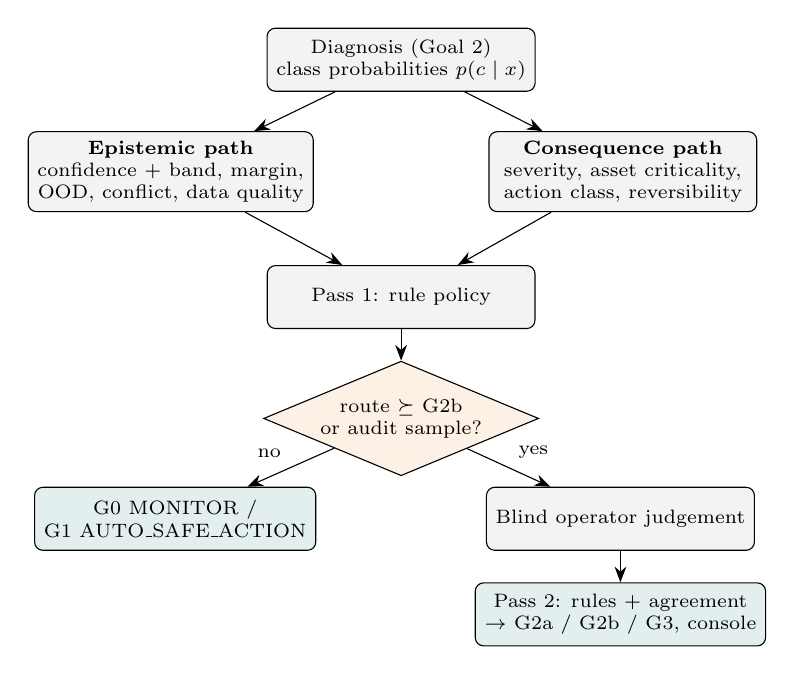
\begin{tikzpicture}[
  b/.style={draw,rounded corners=3pt,align=center,font=\scriptsize,minimum width=34mm,minimum height=8mm,fill=blue!6},
  g/.style={b,fill=green!12}, d/.style={draw,diamond,aspect=2.4,align=center,font=\scriptsize,fill=orange!12,inner sep=1pt},
  >={Stealth[length=2mm]}, node distance=4mm and 8mm]
\node[b] (dia) {Diagnosis (Goal 2)\\ class probabilities $p(c\mid x)$};
\node[b,below left=5mm and -6mm of dia] (ep) {\textbf{Epistemic path}\\ confidence + band, margin,\\ OOD, conflict, data quality};
\node[b,below right=5mm and -6mm of dia] (cp) {\textbf{Consequence path}\\ severity, asset criticality,\\ action class, reversibility};
\node[b,below=22mm of dia] (p1) {Pass 1: rule policy};
\node[d,below=of p1] (q) {route $\succeq$ G2b\\ or audit sample?};
\node[g,below left=5mm and 2mm of q] (g01) {G0 MONITOR /\\ G1 AUTO\_SAFE\_ACTION};
\node[b,below right=5mm and 2mm of q] (blind) {Blind operator judgement};
\node[g,below=of blind] (p2) {Pass 2: rules + agreement\\ $\to$ G2a / G2b / G3, console};
\draw[->] (dia)--(ep); \draw[->] (dia)--(cp); \draw[->] (ep)--(p1); \draw[->] (cp)--(p1); \draw[->] (p1)--(q);
\draw[->] (q)--node[above left,font=\scriptsize]{no}(g01); \draw[->] (q)--node[above right,font=\scriptsize]{yes}(blind);
\draw[->] (blind)--(p2);
\end{tikzpicture}
\caption{Runtime decision flow. The epistemic and consequence paths stay separate until the policy is applied, so
confidence cannot dilute risk; the blind judgement comes before final routing because agreement is an input.}
\end{figure}

\paragraph{Inputs.} From Goal~2, per flagged meter-day: the calibrated probability of each of \NORM, \GE, \MF{}
and \SD, the band and the rule that fired; from Goal~1, the anomaly score, the neighbourhood support and the
feeder-balance alarm. \ND{} (communication loss) is handled by rule R0. In N1 the classes cover 37 genuine
events, 33 meter faults, 8 falsifications and 20 communication losses.

\paragraph{Five quantities that must not be merged.} Anomaly score (how unusual), AI confidence (how sure),
severity (how significant technically), asset criticality (how important the asset) and risk (what happens if the
governance decision is wrong). Only risk is derived from the others, by an explicit rule.

\begin{table}[H]
\centering\small
\caption{Asset criticality and severity. The dataset has no critical asset and no criticality or severity field;
both are a documented synthetic overlay, joined on identifiers without modifying the data.}
\begin{tabularx}{\textwidth}{@{}>{\raggedright\arraybackslash}p{6.2cm}>{\raggedright\arraybackslash}p{2.0cm}L@{}}
\toprule\hdr
\textbf{Asset (registry \texttt{configs/assets.yaml})} & \textbf{Criticality} & \textbf{In N1} \\
\midrule
Residential meter & LOW & 24 meters \\
Small commercial meter & MEDIUM & 6 meters (F1: 2, F2: 3, F3: 1) \\
Feeder-head meter, feeder switching & HIGH & 3 feeders \\
Feeder N1-F3 (assumed to supply a health centre) & CRITICAL & 10 meters \\
\midrule
\textbf{Scope and duration} & \textbf{Severity} & \\
\midrule
One meter, less than 6 hours & LOW & \\
One meter for 6 hours or more, or 2--6 meters & MEDIUM & \\
A whole feeder (10 meters) & HIGH & \\
The whole node or the transformer & CRITICAL & \\
\bottomrule
\end{tabularx}

\end{table}

\begin{table}[H]
\centering\footnotesize
\caption{Governance levels. G0--G1 are ``AI handles''; G2a--G3 are ``defer''. Above G1, only G1 actions may run
automatically; locked actions never run on timeout.}
\begin{tabularx}{\textwidth}{@{}>{\raggedright\arraybackslash}p{0.8cm}>{\raggedright\arraybackslash}p{3.3cm}>{\raggedright\arraybackslash}p{3.1cm}L@{}}
\toprule\hdr
\textbf{Level} & \textbf{Route} & \textbf{Who decides} & \textbf{Typical case} \\
\midrule
G0 & MONITOR & AI & \NORM, confident, familiar \\
G1 & AUTO\_SAFE\_ACTION & AI (whitelisted reversible, non-physical actions) & confident freeze of a residential meter \\
G2a & AI\_RECOMMENDATION & AI proposes, operator acknowledges & probable meter fault, inspection suggested \\
G2b & HUMAN\_REVIEW & operator, after blind judgement & uncertainty, disagreement, OOD, suspicious data, high risk \\
G3 & HUMAN\_APPROVAL\_REQUIRED & named operator with written justification (two people if risk is CRITICAL) & switching, disconnection, fraud declaration, critical asset \\
\bottomrule
\end{tabularx}

\end{table}

\subsection{Risk and confidence}
\paragraph{Confidence bands.} With $\hat c=\arg\max_c p(c\mid x)$ and $p^\star=p(\hat c\mid x)$, the band is HIGH
if $p^\star\ge\tau^{\mathrm{high}}_{\hat c}$, LOW if $p^\star<\tau^{\mathrm{low}}_{\hat c}$, MEDIUM otherwise
($\tau^{\mathrm{high}}=0.90$, $0.85$ for \GE; $\tau^{\mathrm{low}}=0.60$; minimum margin $p_{(1)}-p_{(2)}=0.30$). The band
is capped at MEDIUM when the input is out of distribution, data quality is not good, or the class's calibration
is not validated --- which requires at least 30 out-of-fold events. In N1 this holds for \GE{} (37) and \MF{} (33)
but not \SD{} (8), so every suspicious-data case is reviewed by a human.

\paragraph{Risk.} The wrong-action risk of an action $a$ on an asset of criticality $\kappa$ is
$\rho_{\mathrm{act}}(a)=\max(\beta(a)\oplus\mathbb 1_{\mathrm{irrev}}(a),\kappa)$ for physical or customer-affecting
actions and $\beta(a)\oplus\mathbb 1_{\mathrm{irrev}}(a)$ otherwise, with $\beta(a)$ the base risk of the action
class and $\oplus1$ one level up. The missed-event risk uses the most severe \emph{plausible} hypothesis, so a
confident \MF{} cannot hide a plausible \GE:
\begin{equation}
\sigma^\star(x)=\max_{c:\,p(c\mid x)\ge0.05}\sigma(c),\qquad \rho_{\mathrm{miss}}=M[\kappa,\sigma^\star],\qquad
\rho_{\mathrm{case}}=\max\bigl(\rho_{\mathrm{miss}},\max_a\rho_{\mathrm{act}}(a)\bigr),
\end{equation}
where $M$ is an ordinal criticality $\times$ severity matrix (e.g.\ LOW criticality with HIGH severity gives
MEDIUM risk; CRITICAL criticality with HIGH severity gives CRITICAL). A maximum is used, never a weighted sum:
ordinal ranks cannot be averaged, and ``low severity'' must never cancel ``health-centre feeder''. The price is
over-escalation, which is measured rather than assumed acceptable.

\subsection{Escalation policy}
Order the routes $\mathrm{G0}\prec\mathrm{G1}\prec\mathrm{G2a}\prec\mathrm{G2b}\prec\mathrm{G3}$; each rule sets a
floor and $\mathrm{route}(e)=\max_k f_k(e)$.

\begin{table}[H]
\centering\footnotesize
\caption{Routing rules. R6 follows the dataset's reference responses: a drift or bias that bills a customer
wrongly for weeks needs a human; scheduled load shedding and short sags only need logging.}
\begin{tabularx}{\textwidth}{@{}>{\raggedright\arraybackslash}p{1.9cm}LL>{\raggedright\arraybackslash}p{1.3cm}@{}}
\toprule\hdr
\textbf{Rule} & \textbf{Condition} & \textbf{Floor / effect} & \textbf{Tunable} \\
\midrule
R0 Input validity & missing inputs (\ND), unregistered asset, unapproved model & $\ge$ G2b; short communication loss ($\le$12 intervals): G1 gap filling & no \\
R1 Hard action & physical, customer-affecting, accusatory or irreversible action & action locked; G3 & no \\
R2 Consequence & case risk CRITICAL, or CRITICAL asset with a non-\NORM{} diagnosis & $\ge$ G2b, consequential actions locked, two-person approval if CRITICAL & no \\
R2b & case risk HIGH & $\ge$ G2b & no \\
R3 Agreement & strong / partial disagreement, weak agreement & $\ge$ G2b (+ second review, more data, freeze if strong) & no \\
R4 Familiarity & out of distribution, insufficient data & $\ge$ G2b + more data & thresholds \\
R5 Confidence & LOW band or strong conflict / MEDIUM band or small margin & $\ge$ G2b / $\ge$ G2a & yes \\
R6 Diagnosis default & \NORM{} $\to$ G0. \MF{} $\to$ G1, $\ge$ G2a for a voltage offset or clock shift, $\ge$ G2b if it lasts 24~h or more or affects billing (gain drift, bias). \GE{} $\to$ G0 if scheduled or self-clearing (load shedding, short sag, surge), G2a otherwise, $\ge$ G2b for an equipment cause of severity $\ge$ MEDIUM. \SD{} $\to$ G2b & floor & yes \\
R7 Recurrence & too many automatic actions on one asset & $\ge$ G2b & yes \\
R8 Workload & queue strained & priority only, never the route & yes \\
R9 Consistency & locked action $\to$ G3; proposed action $\to$ $\ge$ G2a & floor & no \\
\bottomrule
\end{tabularx}

\end{table}

\paragraph{Critical consequence dominates confidence.} For any non-\NORM{} diagnosis, every hard action is locked
and routed to G3, and a CRITICAL asset is always at least G2b, \emph{for every value of the AI confidence}:
R1, the criticality branch of R2 and R9 do not depend on $p^\star$, and a maximum of floors cannot be lowered by
the floors that do. Confidence may resolve doubt about \emph{what happened}, never change \emph{what is at stake}.
The property is an automated test on 400 random cases (\texttt{tests/test\_governance.py}).

\paragraph{Two passes and agreement.} Pass~1 applies every rule except R3; if the route is G2b or above, or the
case falls in the 5\% audit sample, the operator gives a blind diagnosis and a LOW/MID/HIGH confidence. Pass~2
adds R3, which can only raise the route. Agreement states: AGREEMENT (same class, both at least MID; never lowers
the route), WEAK\_AGREEMENT (same class, someone guessing; $\ge$ G2b + more data), PARTIAL (competing hypotheses;
$\ge$ G2b) and STRONG (different classes, the AI gives the operator's class less than 0.20, and both are confident
or the pair is critical, e.g.\ \GE{} vs.\ \MF; $\ge$ G2b + second review + more data + freeze). When neither party
is confident, at most two rounds of safe data requests (neighbour readings, feeder-head voltage, history, feeder
balance) are run before a supervisor takes the case; new evidence may raise the route, never lower it.

\subsection{Operator interaction and audit}
\begin{figure}[htbp]
\centering
\begin{lstlisting}[basicstyle=\ttfamily\scriptsize,breaklines=false]
PHASE 1 - BLIND ASSESSMENT                PHASE 2 - REVEAL AND DECIDE
+-------------------------------------+   +------------------------------------------+
| Evidence only: trends, neighbours,  |   | Your view (locked)   | AI view           |
| data quality, severity, criticality |   | GENUINE_EVENT  HIGH  | METER_FAULT  HIGH |
| (AI diagnosis hidden)               |   |                      | right in 30 of 33 |
| Your diagnosis: [GENUINE_EVENT]     |   |                      | validation events |
| Your confidence: LOW / MID / HIGH   |   | !! STRONG DISAGREEMENT - actions locked  |
| [Submit, show AI view]              |   | [APPROVE] [OVERRIDE] [MORE DATA] [2ND]   |
+-------------------------------------+   +------------------------------------------+
\end{lstlisting}
\caption{Operator console mock-up: blind assessment first, then the AI's view is revealed (counts illustrative).}
\label{fig:console}
\end{figure}
\textbf{Against over-trust:} blind-first judgement; confidence as a band with its real validation count, and no
count at all where calibration is not validated (on N1: \SD); the runner-up always shown; equal buttons with no
default; written justification for G3 approvals and overrides; two-person approval for CRITICAL risk.
\textbf{Against under-trust:} routine events never reach the operator; track records of AI and operators per event
type; outcome feedback; similar past incidents.

Every decision is appended to the hash-chained decision log shared with Goal~2, as a \texttt{governance} block
(severity, criticality, per-action risk, blind and post-reveal judgements, agreement, route and fired rules, final
decision and justification, policy version). The expert label used for learning is the \emph{blind} judgement
(the post-reveal one echoes the AI), and the operator's decision is never treated as ground truth. A calibration
phase replays labelled dataset events to estimate each operator's accuracy per class, with Wilson intervals.

\paragraph{Implementation.} The Version~1 engine (bands, risk, agreement, locks, routing R0--R9) is
\texttt{src/energymind/govern/policy.py}; the six scenarios below and five safety invariants, each on 400 random
cases, are automated tests. The request-more-data loop, the console and Version~2 are design.

\paragraph{Version 2.} A learned rejector replaces only the tunable rules R5--R6, inside the immutable rules:
$\mathrm{route}_{V2}(e)=\max\bigl(\max_{k\in\{R0,R1,R2,R3,R9\}}f_k(e),\ \phi(r_\theta(x))\bigr)$ with
$\phi=\mathrm{G1}$ (AI handles) or G2b (defer). It can only move cases inside the region the rules already allow to
automate, and is promoted only after a shadow-mode comparison with Version~1.

\subsection{Evaluation}
The layer is evaluated as a human--AI system on N1's labelled event stream, with synthetic operator profiles and
AI outputs taken out-of-fold from Goal~2. Main metrics: coverage $|A|/N$; review rate; false-escalation rate
(deferred although the AI was right and the risk was low); missed-escalation rate (automated although the AI was
wrong or the risk required review); unsafe automatic actions (must be exactly 0); system accuracy and a
cost-weighted loss; over- and under-reliance; decision time and workload. Two analyses follow the references: a
coverage sweep (system accuracy and missed escalations against coverage, one curve per operator profile) and an
alignment audit (positive rate per AI-confidence bin and operator level; cells with at least 30 samples, which N1
reaches only for \GE{} and \MF). The out-of-distribution rule is exercised on N1's hard-negative periods
(Ramadan, August vacations) and on its clock shift, which Goal~1 does not recognise.

\paragraph{Agreement with the dataset's reference policy.} Each labelled reading carries a suggested response,
which we defined in our data card as a starting point; each route is compared with it, a route below the reference
counting as a missed escalation and above it as a false escalation. Deviations caused by the asset overlay (a sag
on the critical feeder is reviewed although the reference says ``log'') are listed separately.

\begin{table}[H]
\centering\small
\caption{Reference responses and their nearest governance level.}
\begin{tabularx}{\textwidth}{@{}>{\raggedright\arraybackslash}p{3.0cm}>{\raggedright\arraybackslash}p{2.0cm}L@{}}
\toprule\hdr
\textbf{Reference response} & \textbf{Route} & \textbf{N1 readings} \\
\midrule
\texttt{auto\_log} & G0 & 1\,100 grid-event and 50 equipment readings (load shedding, sag, surge, cold-load pickup) \\
\texttt{auto\_correct} & G1 & 112 corruption, 151 stuck meter, 78 short communication losses \\
\texttt{notify\_operator} & G2a & 500 outage/swell, 3\,711 voltage-offset/clock-shift, 351 long communication losses \\
\texttt{human\_decision} & $\ge$ G2b & 14\,175 falsification, 8\,922 gain drift/bias, 3\,244 equipment failure \\
\bottomrule
\end{tabularx}

\end{table}

\begin{table}[H]
\centering\footnotesize
\caption{Reference scenarios built on real N1 events, run as automated tests in \texttt{tests/test\_governance.py} (AI outputs and operator answers are scripted test inputs).
S2 and S6 show the central claim: high confidence, even with human agreement, never authorises a consequential or
accusatory action.}
\begin{tabularx}{\textwidth}{@{}>{\raggedright\arraybackslash}p{3.1cm}>{\raggedright\arraybackslash}p{2.6cm}L>{\raggedright\arraybackslash}p{1.8cm}@{}}
\toprule\hdr
\textbf{Scenario (N1 event)} & \textbf{AI output (scripted)} & \textbf{Outcome} & \textbf{Reference} \\
\midrule
S1 Stuck meter, N1-F1, 12--14 Feb & \MF{} 0.95 & automatic safe action (quarantine, re-read, ticket); review if it outlasts 24~h & auto\_correct \\
S2 Voltage sag on the critical feeder N1-F3, 27 Jun & \GE{} 0.98 & transfer to backup feeder locked: two-person approval & auto\_log (overlay) \\
S3 Gain drift, N1-F2, from 19 Apr & \MF{} 0.92, operator agrees & human review (billing); agreement does not lower it & human\_decision \\
S4 Demand surge, N1-F2, 23 Jun & \MF{} 0.93 vs.\ operator \GE{} & strong disagreement: second review, more data, freeze & auto\_log \\
S5 Clock shift, N1-F1, 23 Feb & \SD{} 0.46, OOD & review with a request for more data; no consequential action & notify\_operator \\
S6 Partial bypass, N1-F2, 4 Feb & \SD{} 0.94, capped at MEDIUM & disconnection locked: two-person approval; operator orders an inspection & human\_decision \\
\bottomrule
\end{tabularx}

\end{table}

\paragraph{Limitations.} No real operator data (thresholds, risk matrix and agreement rules are engineering
choices); synthetic criticality; only 8 suspicious-data events in N1, so their calibration cannot be validated;
conservative by design; the policy decides which cases humans see, so logged data reflect the policy (the audit
sample mitigates this); blind-phase latency may be too slow for urgent cases; an attacker aware of the policy could
try to stay inside the automated region. All results are simulated and must be reported as such.

\clearpage
% generated by build_parts.py from the goal report -- edit the report, not this file
\section{Goal 4: Shared Learning Across the Noosphere}
\label{g4-sec:goal4}

\subsection{Why a single node is not enough}

A neighborhood node sees only a few examples of each failure mode. In our simulated year, each falsification type occurs only 2--3 times \emph{in the whole dataset}, that is at most once per node, and several types never occur in a given node at all (Table~\ref{g4-tab:pernode}). The hardest cases for a lone detector (\code{selective\_bypass}, \code{partial\_reduction\_bypass}, \code{meter\_zeroing}, \code{gain\_drift}, \code{clock\_shift}, \code{negative\_value}, \code{transformer\_degradation}) are exactly the rare ones; the Goal~1 run on node N1 confirms that bypasses, biases and drifts are the cases a single node detects worst. A node that has never seen an attack cannot recognise it; a node that has will recognise it earlier if its neighbours warn it.

\begin{table}[H]
\centering\small
\caption{Falsification events per node in the dataset. A 0 means the node never sees that attack in the year.}
\label{g4-tab:pernode}
\begin{tabular}{@{}l ccc@{}}
\toprule\hdr
Falsification type & N1 & N2 & N3 \\
\midrule
\code{coordinated\_fdi} & 1 & \textbf{0} & 1 \\
\code{fdi\_evasion} & 1 & 1 & \textbf{0} \\
\code{fdi\_inflate} & 1 & \textbf{0} & 1 \\
\code{fdi\_replay} & 1 & \textbf{0} & 1 \\
\code{fdi\_scale} & 1 & 1 & \textbf{0} \\
\code{meter\_zeroing} & 1 & 1 & \textbf{0} \\
\code{partial\_reduction\_bypass} & 1 & 1 & 1 \\
\code{selective\_bypass} & 1 & \textbf{0} & 1 \\
\bottomrule
\end{tabular}
\end{table} Goal~4 turns the local trust layer of Goals~1--3 into a \emph{collective immune system}: nodes exchange what they \emph{learned}, never what they \emph{measured}.

The design rests on three principles:
\begin{enumerate}[label=\textbf{P\arabic*.}]
  \item \textbf{Share knowledge, not data.} Raw readings, identifiers, explanations and logs never leave the node.
  \item \textbf{Trust nothing shared by default.} Every incoming artifact is treated like an unverified meter reading: it is validated, canary-tested locally, and adopted only with operator approval.
  \item \textbf{Sharing can never trigger grid action.} The escalation rules of Goal~3 stay in force whatever the shared model says; shared knowledge only changes \emph{scores}, never \emph{authority}.
\end{enumerate}

\subsection{Nodes and honest scope}

The evaluation uses our simulated dataset (1{,}051{,}200 half-hourly rows, 60 meters, 7 feeders, seed 2025). Each node is one smart-metered neighborhood (Table~\ref{g4-tab:nodes}); public Tunisian statistics were used only to calibrate the simulator, so no result here describes a real STEG grid. Node N1 is the Phase~1 single-node prototype on which Goals~1--3 run; N2 and N3 are the other participants of the sharing design. As the challenge allows, multi-node sharing is a documented design in Phase~1: the protocol below is specified, and the experiments that would measure its benefit are planned in Section~\ref{g4-sec:eval}.

\begin{table}[H]
\centering\small
\caption{Simulated nodes. Heterogeneity (climate, meter mix, feeder length, customer class) is what makes sharing useful; a common simulator limits how large it is.}
\label{g4-tab:nodes}
\begin{tabularx}{\textwidth}{@{}l Y r r Y@{}}
\toprule\hdr
Node & Profile & Meters & Feeders & Role in the experiments \\
\midrule
N1 & Coastal suburb & 30 & 3 & Largest node; local-baseline reference \\
N2 & Hot interior town & 15 & 2 & Strong summer load, different climate regime \\
N3 & Mixed residential/commercial & 15 & 2 & Different customer classes and load shapes \\
\bottomrule
\end{tabularx}
\end{table}

\subsection{Architecture of the Noosphere}

Figure~\ref{g4-fig:arch} shows the architecture. Each node runs the full local trust pipeline and exposes only three narrow, versioned \emph{channels} to a coordinator. A fourth, out-of-band \emph{alert} path carries urgent attack warnings.

\begin{figure}[H]
\centering
\resizebox{\textwidth}{!}{%
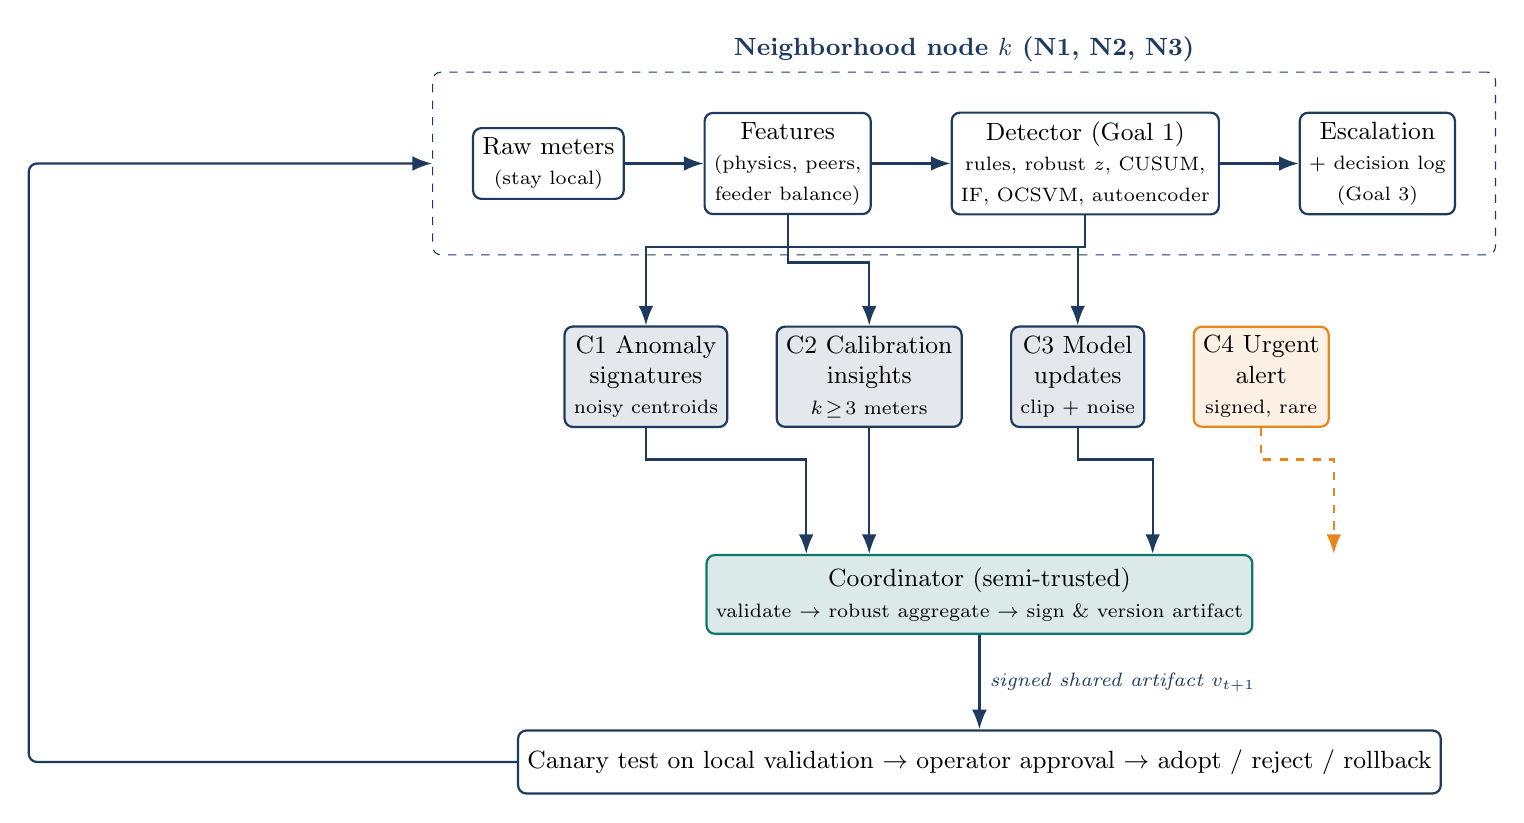
\begin{tikzpicture}[
  node distance=6mm and 10mm,
  box/.style={rectangle,rounded corners=3pt,draw=emblue,fill=emgrey,thick,align=center,minimum height=8mm,font=\small},
  local/.style={box,fill=white},
  chan/.style={box,fill=emblue!12},
  coord/.style={box,fill=emgreen!15,draw=emgreen,minimum height=10mm},
  arr/.style={-{Latex[length=2.5mm]},thick,emblue},
  warn/.style={-{Latex[length=2.5mm]},thick,emorange,dashed},
  lbl/.style={font=\scriptsize\itshape,emblue}]
% node stack
\node[local] (data) {Raw meters\\\scriptsize (stay local)};
\node[local,right=of data] (feat) {Features\\\scriptsize (physics, peers,\\\scriptsize feeder balance)};
\node[local,right=of feat] (det) {Detector (Goal 1)\\\scriptsize rules, robust $z$, CUSUM,\\\scriptsize IF, OCSVM, autoencoder};
\node[local,right=of det] (esc) {Escalation\\\scriptsize + decision log\\\scriptsize (Goal 3)};
\draw[arr] (data)--(feat); \draw[arr] (feat)--(det); \draw[arr] (det)--(esc);
\begin{scope}[on background layer]
 \node[draw=emblue,dashed,rounded corners=3pt,fit=(data)(feat)(det)(esc),inner sep=5mm,
       label={[font=\small\bfseries,emblue]above:Neighborhood node $k$ (N1, N2, N3)}] (nodebox) {};
\end{scope}
% channels
\node[chan,below=14mm of feat,xshift=-18mm] (c1) {C1 Anomaly\\ signatures\\\scriptsize noisy centroids};
\node[chan,right=6mm of c1] (c2) {C2 Calibration\\ insights\\\scriptsize $k\!\ge\!3$ meters};
\node[chan,right=6mm of c2] (c3) {C3 Model\\ updates\\\scriptsize clip + noise};
\node[chan,right=6mm of c3,draw=emorange,fill=emorange!12] (c4) {C4 Urgent\\ alert\\\scriptsize signed, rare};
\draw[arr] (det.south)--++(0,-4mm)-|(c1.north);
\draw[arr] (det.south)--++(0,-4mm)-|(c3.north);
\draw[arr] (feat.south)--++(0,-6mm)-|(c2.north);
% coordinator
\node[coord,below=16mm of c2,xshift=14mm] (co) {Coordinator (semi-trusted)\\\scriptsize validate $\to$ robust aggregate $\to$ sign \& version artifact};
\draw[arr] (c1.south)--++(0,-4mm)-|([xshift=-22mm]co.north);
\draw[arr] (c2.south)--(c2.south|-co.north);
\draw[arr] (c3.south)--++(0,-4mm)-|([xshift=22mm]co.north);
\draw[warn] (c4.south)--++(0,-4mm)-|([xshift=45mm]co.north);
% return
\node[local,below=12mm of co] (canary) {Canary test on local validation $\to$ operator approval $\to$ adopt / reject / rollback};
\draw[arr] (co)--node[lbl,right]{signed shared artifact $v_{t+1}$}(canary);
\draw[arr,rounded corners=3pt] (canary.west)--++(-62mm,0)|-(nodebox.west);
\end{tikzpicture}}
\caption{Noosphere architecture. Raw data and decisions stay inside the node; three protected channels and one urgent-alert path reach a coordinator, whose output is only adopted after a local canary test and human approval.}
\label{g4-fig:arch}
\end{figure}

\subsection{What is shared, what stays local, and why}

\begin{table}[H]
\centering\small
\caption{Sharing contract. Each row answers the challenge's three questions: what, what stays local, why.}
\label{g4-tab:sharing}
\begin{tabularx}{\textwidth}{@{}p{2.1cm} Y Y Y@{}}
\toprule\hdr
Channel & Shared artifact & Safeguards & Why it helps \\
\midrule
\textbf{C1} Anomaly patterns & Per-node centroids of ``trusted'' and ``untrusted'' records in a robustly standardised feature space (Eq.~\ref{g4-eq:protocol-preprocessing}); optional per-\emph{family} centroids when $\ge n_{\min}$ events exist: physical bypass and data-only FDI (Goal~2 verdict \code{SUSPICIOUS\_DATA}), sensor drift and corruption (\code{METER\_FAULT}) & Feature clipping, Gaussian noise on released centroids, coordinate-wise median across nodes, count bucketing & Lets a node recognise an attack family it has seen too rarely to learn, without exchanging any time series \\
\addlinespace
\textbf{C2} Calibration insights & Median of $\log\!\big(E/(V\,I\,\mathrm{PF}\,\Delta t/1000)\big)$ per \emph{meter model} on clean, non-exporting readings, with sample size bucket & Release a model only if $\ge 3$ meters contribute; medians only; no meter IDs & Separates a model-wide calibration bias (firmware, batch) from a single faulty meter \\
\addlinespace
\textbf{C3} Model updates & Clipped, noised updates to a shared logistic-regression screening model & Update-norm clipping $C$, Gaussian noise $\sigma$, robust aggregation, secure aggregation (deployment) & Nodes with few rare events borrow strength from others; the shared model supports, never replaces, the local detectors of Goal~1 \\
\addlinespace
\textbf{C4} Urgent alert & Signed ``attack fingerprint'': subtype family, feature-residual profile, affected meter-model, severity & Human-confirmed at the source node; rate-limited; expires; receivers treat it as a \emph{prior}, not a verdict & Days-to-hours propagation of a confirmed coordinated attack \\
\bottomrule
\end{tabularx}
\end{table}

\paragraph{Stays local (never leaves the node):} raw readings and timestamps; meter, customer and feeder identifiers; coordinates and dwelling data; per-meter reference values and the local median/MAD scaling statistics; per-record features, verdicts and SHAP explanations; operator notes and overrides; full decision logs; local detector models. \emph{Reason:} half-hourly smart-meter traces reveal occupancy, sleep and appliance use~\cite{hart1992,molina2010}; explanations and logs are accountability records that belong to the operator that made the decision.

\subsection{Protocol}
\label{g4-subsec:protocol}

The protocol defines how independent neighborhood nodes prepare local
information, share privacy-aware summaries or model updates, and evaluate
the knowledge received from the coordinator. Raw meter readings and
record-level decisions remain local. The protocol distinguishes four
sharing channels: anomaly signatures (C1), calibration insights (C2),
federated model updates (C3), and urgent alerts (C4). C1--C3 are regular
knowledge-sharing mechanisms, whereas C4 is a separate, rare alert path.

\subsubsection{Protocol overview}

Figure~\ref{g4-fig:protocol-pipeline} presents the complete protocol, from
local data preparation to the local acceptance or rejection of a shared
model. The multi-node communication and secure aggregation components
are documented design requirements; the figure describes the proposed
architecture rather than claiming that the complete distributed system
has been deployed.

\begin{figure}[H]
\centering
\resizebox{\textwidth}{!}{%
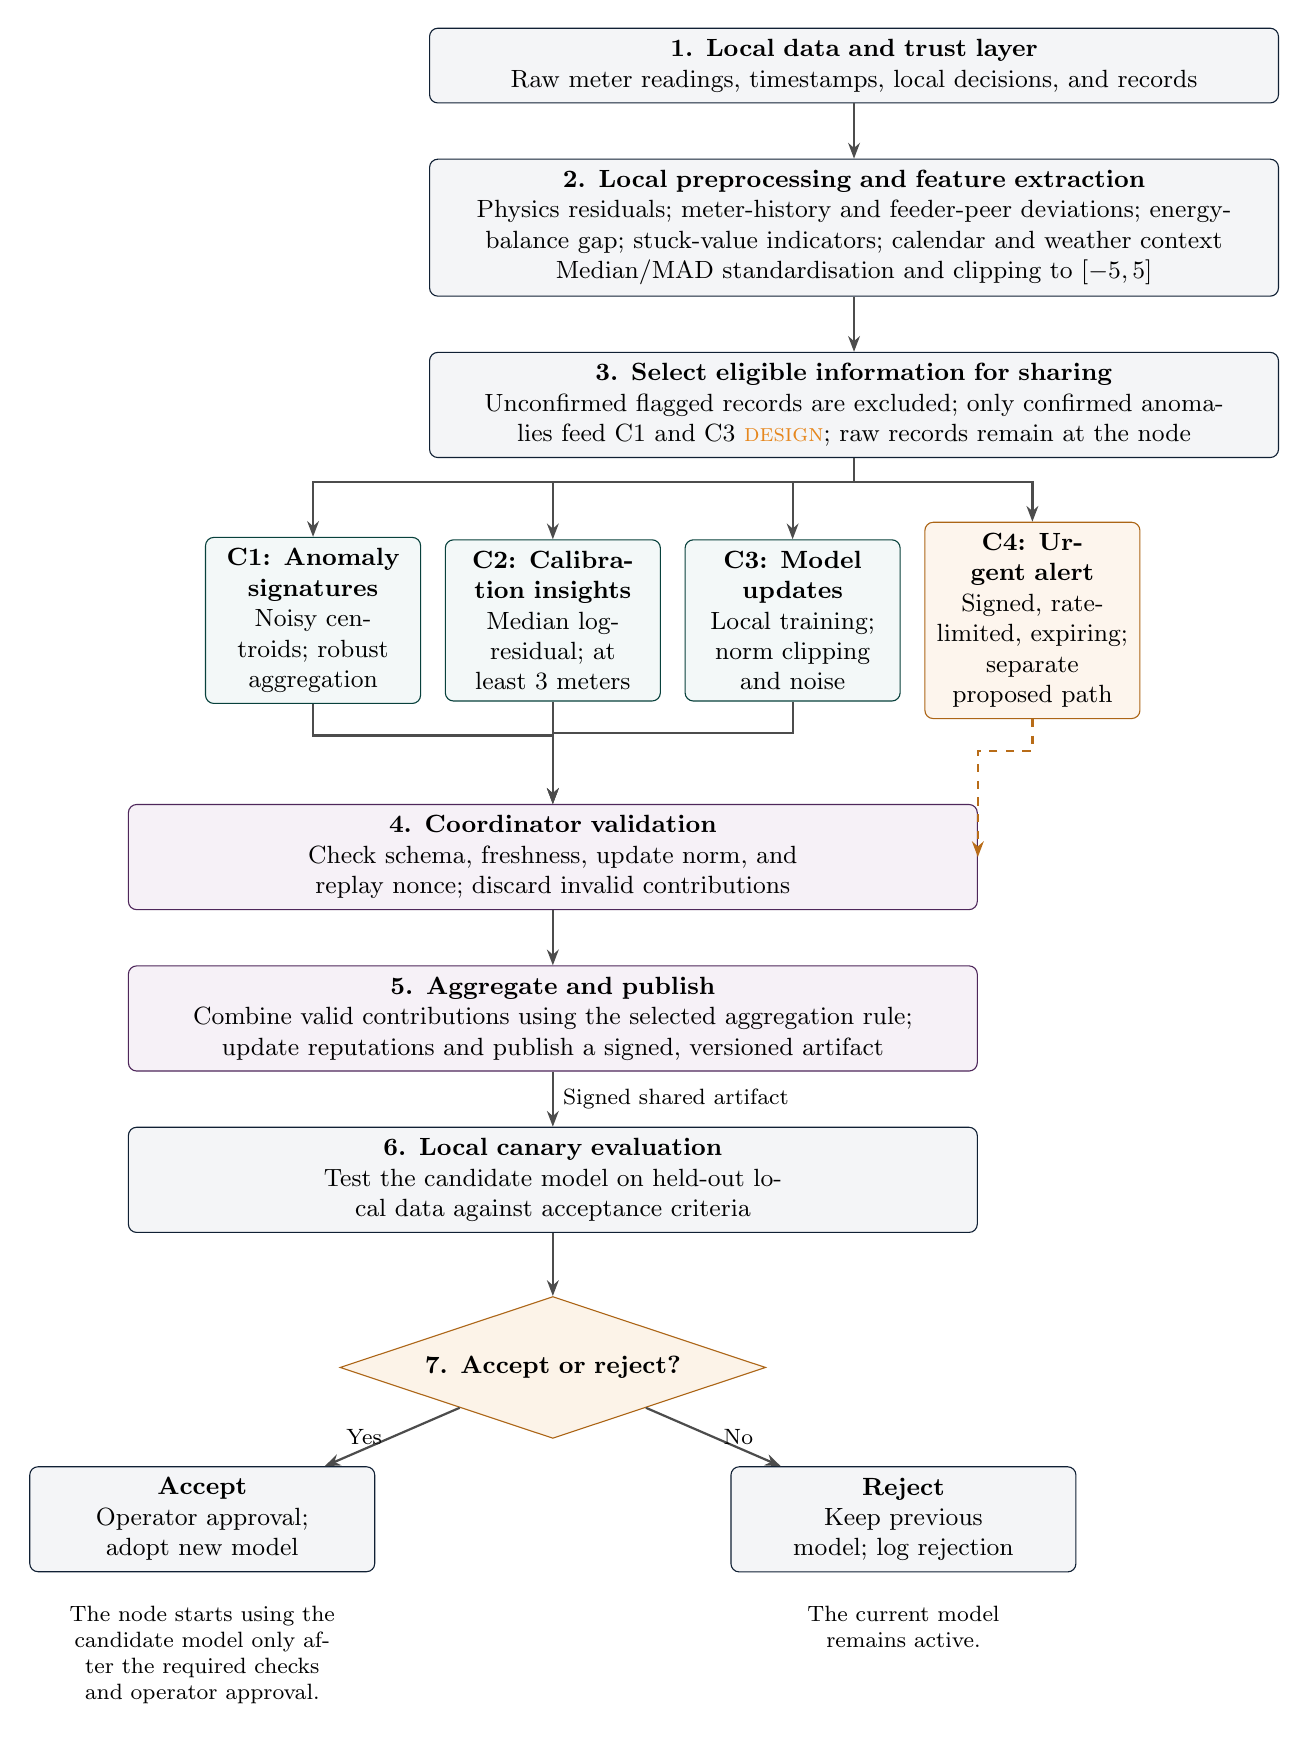
\begin{tikzpicture}[
    font=\small,
    node distance=7mm,
    process/.style={
        rectangle, rounded corners=3pt,
        draw=blue!55!black, fill=blue!5,
        text width=10.5cm, align=center,
        minimum height=9mm, inner sep=4pt
    },
    channel/.style={
        rectangle, rounded corners=3pt,
        draw=teal!55!black, fill=teal!5,
        text width=2.45cm, align=center,
        minimum height=16mm, inner sep=4pt
    },
    coordinator/.style={
        rectangle, rounded corners=3pt,
        draw=violet!65!black, fill=violet!7,
        text width=10.5cm, align=center,
        minimum height=12mm, inner sep=4pt
    },
    decision/.style={
        diamond, aspect=3.0,
        draw=orange!75!black, fill=orange!10,
        text width=4.0cm, align=center,
        inner sep=2pt
    },
    arr/.style={-{Stealth[length=2mm]}, thick, draw=black!70},
    note/.style={font=\footnotesize, align=center}
]

\node[process] (local) {
    \textbf{1. Local data and trust layer}\\
    Raw meter readings, timestamps, local decisions, and records
};

\node[process, below=of local] (prep) {
    \textbf{2. Local preprocessing and feature extraction}\\
    Physics residuals; meter-history and feeder-peer deviations;
    energy-balance gap; stuck-value indicators; calendar and weather context\\
    Median/MAD standardisation and clipping to $[-5,5]$
};

\node[process, below=of prep] (select) {
    \textbf{3. Select eligible information for sharing}\\
    Unconfirmed flagged records are excluded; only confirmed anomalies
    feed C1 and C3 \design{}; raw records remain at the node
};

\node[channel, below left=10mm and 1mm of select] (c1) {
    \textbf{C1: Anomaly signatures}\\
    Noisy centroids; robust aggregation
};

\node[channel, right=3mm of c1] (c2) {
    \textbf{C2: Calibration insights}\\
    Median log-residual; at least 3 meters
};

\node[channel, right=3mm of c2] (c3) {
    \textbf{C3: Model updates}\\
    Local training; norm clipping and noise
};

\node[channel, right=3mm of c3, draw=orange!75!black,
      fill=orange!8] (c4) {
    \textbf{C4: Urgent alert}\\
    Signed, rate-limited, expiring; separate proposed path
};

\node[coordinator, below=13mm of c2] (validate) {
    \textbf{4. Coordinator validation}\\
    Check schema, freshness, update norm, and replay nonce;
    discard invalid contributions
};

\node[coordinator, below=of validate] (aggregate) {
    \textbf{5. Aggregate and publish}\\
    Combine valid contributions using the selected aggregation rule;
    update reputations and publish a signed, versioned artifact
};

\node[process, below=of aggregate] (test) {
    \textbf{6. Local canary evaluation}\\
    Test the candidate model on held-out local data against acceptance criteria
};

\node[decision, below=of test, yshift=-1mm] (decision) {
    \textbf{7. Accept or reject?}
};

\node[process, below left=8mm and 9mm of decision,
      text width=4.1cm, minimum height=9mm] (accept) {
    \textbf{Accept}\\
    Operator approval; adopt new model
};

\node[process, below right=8mm and 9mm of decision,
      text width=4.1cm, minimum height=9mm] (reject) {
    \textbf{Reject}\\
    Keep previous model; log rejection
};

\draw[arr] (local) -- (prep);
\draw[arr] (prep) -- (select);
\draw[arr] (select.south) -- ++(0,-3mm) -| (c1.north);
\draw[arr] (select.south) -- ++(0,-3mm) -| (c2.north);
\draw[arr] (select.south) -- ++(0,-3mm) -| (c3.north);
\draw[arr] (select.south) -- ++(0,-3mm) -| (c4.north);

\draw[arr] (c1.south) -- ++(0,-4mm) -| (validate.north);
\draw[arr] (c2.south) -- (validate.north);
\draw[arr] (c3.south) -- ++(0,-4mm) -| (validate.north);
\draw[arr, dashed, draw=orange!80!black]
    (c4.south) -- ++(0,-4mm) -| (validate.east);

\draw[arr] (validate) -- (aggregate);
\draw[arr] (aggregate) -- node[right, note]
    {Signed shared artifact} (test);
\draw[arr] (test) -- (decision);
\draw[arr] (decision) -- node[left, note] {Yes} (accept);
\draw[arr] (decision) -- node[right, note] {No} (reject);

\node[note, below=3mm of accept, text width=4.2cm] {
    The node starts using the candidate model only after the required checks
    and operator approval.
};

\node[note, below=3mm of reject, text width=4.2cm] {
    The current model remains active.
};

\end{tikzpicture}%
}
\caption{Proposed shared-learning protocol. Raw readings and
record-level decisions remain local. C1--C3 carry regular shared
information; C4 is a separate proposed urgent-alert path. A shared
model is adopted only after local evaluation and operator approval.}
\label{g4-fig:protocol-pipeline}
\end{figure}

\subsubsection{Step 1: Local preprocessing and feature extraction}

Each node processes its own meter data and constructs a feature vector
describing possible anomalies. The features combine:
\begin{itemize}
    \item physical consistency residuals between measured energy
    $E$ and the estimate $VI\,\mathrm{PF}\,\Delta t$;
    \item deviations from the meter's own historical behaviour;
    \item deviations from peer meters on the same feeder;
    \item the feeder energy-balance gap;
    \item indicators of stuck or repeated values;
    \item calendar and weather context.
\end{itemize}

Since feature scales and distributions may differ between nodes, each
node standardises feature $j$ using its own median and median absolute
deviation (MAD), and clips the result to a bounded interval:
\begin{equation}
z_{ij} =
\operatorname{clip}\!\left(
\frac{x_{ij}-\operatorname{med}_j}
     {1.4826\,\mathrm{MAD}_j},
-c,c
\right),
\qquad c=5.
\label{g4-eq:protocol-preprocessing}
\end{equation}

Here, $x_{ij}$ is feature $j$ for record $i$;
$\operatorname{med}_j$ is the local median of feature $j$;
$\mathrm{MAD}_j$ is its median absolute deviation; and
$\operatorname{clip}(u,-c,c)$ restricts $u$ to the interval
$[-c,c]$. The factor $1.4826$ is a conventional scaling factor for
the MAD. The operation limits the influence of extreme feature values
on subsequent shared statistics.

Two kinds of local records are kept apart \design{}. Records that the
local trust layer has flagged but no one has confirmed are excluded from
everything that is shared, so an unverified anomaly can neither distort
the shared picture of normal behaviour nor be presented as an attack.
Records whose cause is confirmed (by an operator, or in the prototype by
the dataset labels \code{gt\_*}) are the \emph{only} anomalies used for
the ``untrusted'' and family centroids of C1 and for the screening model
of C3. This is a documented design rule and should not be interpreted as
proof that the complete multi-node exclusion mechanism has been deployed.

\subsubsection{Step 2: Prepare the information to be shared}

After local preprocessing, a node prepares the relevant artifact for
the selected sharing channel. The four channels serve different
purposes and must not be treated as interchangeable.

\paragraph{C1: Anomaly signatures.}

C1 shares compact representations of anomaly patterns, using centroids
of trusted and untrusted records in the standardised feature space.
When enough examples are available, centroids may also be maintained
for anomaly families such as physical bypass, data-only false data
injection (FDI), and sensor drift.

Before release, centroids use feature clipping and Gaussian noise;
the coordinator combines the received summaries using coordinate-wise
medians. Count bucketing is also specified as a safeguard. This allows
nodes to learn from patterns observed elsewhere without exchanging
individual meter time series.

\paragraph{C2: Calibration insights.}

C2 shares a robust summary of the calibration behaviour of a meter
model. For node $k$ and meter model $m$, the summary is released only
when at least three meters of that model are available locally,
$n_{k,m}\geq 3$:
\begin{equation}
\widetilde r_{k,m}
=
\operatorname{med}_{i\in m}
\operatorname{med}_{t}
\log\!\left(
\frac{E_{it}}
{V_{it} I_{it}\,\mathrm{PF}_{it}\,\Delta t/1000}
\right).
\label{g4-eq:protocol-calibration-local}
\end{equation}

Here, $E_{it}$ is the measured energy for meter $i$ at time $t$;
$V_{it}$ is voltage; $I_{it}$ is current; $\mathrm{PF}_{it}$ is
power factor; and $\Delta t$ is the measurement interval (0.5~h; the
factor 1000 converts W$\cdot$h to kWh). Only clean readings with
$V>0$, no PV export and $E>0$ are used: while a home exports, its
imported energy is 0 and the logarithm is undefined. The inner median
summarises the time-dependent residual for each meter, while the outer
median summarises the meters belonging to model $m$.

The coordinator then takes the median of the summaries received from
eligible nodes:
\begin{equation}
\widetilde r_m
=
\operatorname{med}_{k}\widetilde r_{k,m}.
\label{g4-eq:protocol-calibration-global}
\end{equation}

A value consistently far from zero across several nodes may indicate
a systematic bias associated with that meter model. A deviation
observed for only one meter is more consistent with an individual
meter fault. This is a diagnostic indication, not by itself proof of
the cause.

\emph{On our dataset C2 is a negative control.} The three meter models
differ only by communication technology (GPRS, NB-IoT, PLC), all meters
have accuracy class~1.0, and no model-wide bias was injected. Computed
on the clean data, $\widetilde r_{k,m}$ lies within $\pm0.0002$ (i.e.\
$\pm0.02\%$) for every node and model, so any larger value would be a
false alarm. With the $n_{k,m}\ge3$ rule, the PLC model (5 meters in N1,
none in N2, 2 in N3) is released by N1 only, so its ``median across
nodes'' rests on a single node. A positive test is planned
(Section~\ref{g4-sec:eval}): a $+3\%$ gain is injected on all NB-IoT meters
\emph{inside the experiment code}, leaving the dataset unchanged; C2
must report it, while a single biased meter (\code{bias\_step}) must not
move the model-level value.

\paragraph{C3: Federated model updates.}

C3 allows nodes to contribute to a shared screening model without
transferring their local training records. At round $t$, node $k$
trains the current model $w_t$ on its local dataset $\mathcal D_k$.
The resulting update is
\begin{equation}
\Delta_k
=
\mathrm{LocalTrain}(w_t;\mathcal D_k)-w_t.
\label{g4-eq:protocol-local-update}
\end{equation}

The update $\Delta_k$ represents the change produced by local training.
It is not the raw dataset and does not need to contain individual
meter readings.

\paragraph{C4: Urgent alerts.}

C4 is a separate proposed path for rare, urgent information. An alert
may contain a signed attack fingerprint describing the subtype family,
feature-residual profile, affected meter model, and severity. The
design requires confirmation by a human operator at the source,
rate limiting, and expiration. Receiving nodes should treat the alert
as a prior indication to investigate, not as a definitive verdict.
The full distributed alert path remains a design requirement.

The dataset contains a ready-made case. A \code{coordinated\_fdi}
attack (three meters of one feeder falsified together) hits N3 from
1 to 28~July 2025 and N1 from 14~October 2025. Once N3's operator
confirms the July attack, its fingerprint reaches N1 three months
before N1's own attack. Because Goal~1's physics rule already flags
data-only injection in N1 from the first day, the expected benefit of
the alert is not earlier detection but a faster and more confident
diagnosis: the receiving node can name a confirmed attack family
instead of an unexplained anomaly.

\subsubsection{Step 3: Protect model updates before sharing}

Before a C3 update is shared, the node clips its Euclidean norm and
adds Gaussian noise:
\begin{equation}
\widetilde{\Delta}_k
=
\Delta_k
\min\!\left(1,\frac{C}{\|\Delta_k\|_2}\right)
+
\mathcal N\!\left(
0,\frac{\sigma^2 C^2}{K}I
\right).
\label{g4-eq:protocol-protected-update}
\end{equation}

The symbols have the following meanings:
\begin{itemize}
    \item $C$ is the maximum allowed update norm;
    \item $\|\Delta_k\|_2$ is the Euclidean norm of the local update;
    \item $\sigma$ is the noise multiplier;
    \item $K$ is the number of participating nodes;
    \item $I$ is the identity matrix;
    \item $\mathcal N(0,\frac{\sigma^2 C^2}{K}I)$ is the
    zero-mean Gaussian noise distribution used by the design.
\end{itemize}

If the update norm is no greater than $C$, the clipping factor is
one. If it exceeds $C$, the factor reduces the update until its norm
is $C$. Gaussian noise is then added as a privacy safeguard.

Clipping limits the influence of a single large update, while noise
is intended to reduce the information revealed by the shared update.
However, clipping and adding noise alone do not establish a formal
differential-privacy guarantee. Such a guarantee would require a
specified privacy analysis and accounting procedure.

\subsubsection{Step 4: Validate and aggregate contributions}

The coordinator first checks received contributions against the
announced protocol version and feature schema. It also checks
freshness, update norms, and replay nonces, discarding invalid
contributions. The protocol requires authenticated and encrypted
communication; secure aggregation remains a deployment design
requirement.

For valid C3 updates, the coordinator applies the selected aggregation
rule and updates the shared model:
\begin{equation}
w_{t+1}
=
w_t+
\operatorname{Agg}\!\left(
\widetilde{\Delta}_1,\ldots,
\widetilde{\Delta}_K
\right).
\label{g4-eq:protocol-model-aggregation}
\end{equation}

Here, $\operatorname{Agg}$ is the aggregation function, and
$w_{t+1}$ is the candidate shared model for the next round. Three
aggregation rules are considered.

\paragraph{FedAvg.}

FedAvg takes the arithmetic mean of the protected updates:
\begin{equation}
\operatorname{Agg}_{\mathrm{FedAvg}}
=
\frac{1}{K}\sum_{k=1}^{K}
\widetilde{\Delta}_k.
\label{g4-eq:protocol-fedavg}
\end{equation}

This provides a simple way to combine the contributions of all
participating nodes. However, an unusually large or malicious update
may still affect the average, which motivates robust alternatives.

\paragraph{Coordinate-wise median.}

The coordinator calculates the median separately for each model
coordinate $j$:
\begin{equation}
\left(\operatorname{Agg}_{\mathrm{med}}\right)_j
=
\operatorname{med}_{k}
\left(\widetilde{\Delta}_{k,j}\right).
\label{g4-eq:protocol-coordinate-median}
\end{equation}

Compared with the mean, the coordinate-wise median is less sensitive
to extreme values in individual coordinates. Its robustness has
limits, especially when few nodes participate or several nodes
collude.

\paragraph{Reputation-weighted aggregation.}

The coordinator can also weight updates according to node reputation
and how far each update deviates from the median update:
\begin{equation}
\operatorname{Agg}_{\mathrm{rep}}
=
\sum_{k=1}^{K}\rho_k\widetilde{\Delta}_k,
\qquad
\rho_k\propto r_k\exp\!\left(-\frac{d_k}{\tau}\right),
\label{g4-eq:protocol-reputation-aggregation}
\end{equation}
where
\begin{equation}
d_k =
1-\cos\!\left(
\widetilde{\Delta}_k,\,
\operatorname{med}_{k'}
\widetilde{\Delta}_{k'}
\right).
\label{g4-eq:protocol-update-distance}
\end{equation}

In this expression, $r_k\in[0,1]$ is the reputation of node $k$,
$d_k$ measures the cosine distance between its update and the
coordinate-wise median update, and $\tau$ controls the effect of
that distance on the weight. The proportional weights are normalised
so that they sum to one. Reputation is designed to decrease after
rejected rounds and recover after accepted rounds.

The three aggregation rules are alternatives; they are not three
successive operations that must all be applied to the same update.
The choice of aggregation rule should be stated for each experiment
or deployment configuration.

For C1 anomaly centroids, the coordinator instead applies
coordinate-wise medians to the protected summaries. C2 calibration
summaries are combined using the median across eligible nodes, as
defined in Equation~\ref{g4-eq:protocol-calibration-global}.

\subsubsection{Step 5: Publish the shared artifact}

After validation and aggregation, the coordinator publishes a signed,
versioned artifact containing the relevant shared result. The
coordinator announces the round identifier, protocol version,
feature-schema identifier, clipping and noise parameters $(c,C,\sigma)$,
and deadline. Nodes sign and submit their contributions through the
specified authenticated, encrypted channel.

Versioning allows nodes to identify which shared artifact they have
received. Signatures support integrity and origin verification, while
the validation checks help reject stale or malformed contributions.
These protections describe the intended protocol; they do not imply
that a complete secure multi-node transport and aggregation system
has been implemented.

\subsubsection{Step 6: Local canary evaluation and adoption}

A node does not automatically adopt a newly published model. It first
evaluates the candidate on held-out local canary data and checks the
following criteria:
\begin{itemize}
    \item ROC-AUC must not decrease beyond an allowed margin
    $\Delta_{\mathrm{AUC}}$;
    \item the false-positive rate must remain within the defined alarm
    budget;
    \item genuine \code{grid\_event} and \code{equipment\_failure}
    records must not be misclassified as data-quality problems;
    \item recall per attack \emph{family} (physical bypass, data-only
    FDI, sensor drift, corruption) must not decrease. Per-type recall
    cannot serve as a gate: each falsification type occurs at most once
    per node, so its recall can only be 0 or 1. A family gates adoption
    only where the node holds at least three events of it
    (Table~\ref{g4-tab:canary}); otherwise its result is reported to the
    operator without blocking adoption.
\end{itemize}

\begin{table}[H]
\centering\small
\caption{Events per attack family and node, and whether the family can gate adoption ($\ge3$ events).}
\label{g4-tab:canary}
\begin{tabular}{@{}l ccc@{}}
\toprule\hdr
Family & N1 & N2 & N3 \\
\midrule
Physical bypass & 3 (gate) & 2 & 2 \\
Data-only FDI & 5 (gate) & 2 & 3 (gate) \\
Sensor drift & 8 (gate) & 6 (gate) & 4 (gate) \\
Corruption & 25 (gate) & 14 (gate) & 14 (gate) \\
\bottomrule
\end{tabular}
\end{table}

The numerical thresholds for these criteria must be specified before
deployment. If the candidate passes the checks and receives the
required operator approval, the node adopts it. Otherwise, the node
retains its previous model and logs the rejection.

This local evaluation step limits the risk of adopting a shared model
that is less suitable for a particular neighborhood. It does not,
by itself, prove that the model is safe against every attack or that
the protocol improves detection performance.

\subsubsection{Implementation status and limitations}

The protocol combines local processing, protected information
sharing, robust aggregation, and local model evaluation. Its claims
must nevertheless be interpreted in light of the current
implementation scope:
\begin{itemize}
    \item The experimental data are synthetic; they are not real
    STEG meter readings.
    \item The complete multi-node sharing experiment has not been run.
    The current work does not establish a measured performance
    improvement from cross-node collaboration.
    \item Network transport, node authentication, and secure
    aggregation remain documented design requirements.
    \item The noise mechanisms described here should not be presented
    as a formal differential-privacy guarantee without a complete
    privacy analysis.
    \item Robust aggregation has limitations with a small number of
    participants. With only three nodes, for example, a coordinate-wise
    median cannot guarantee protection against coordinated malicious
    contributions.
\end{itemize}

Accordingly, this section specifies the proposed shared-learning
protocol and its safeguards. What exists as code today are the protocol primitives in
\code{src/energymind/shared/}: update clipping and Gaussian noise
(Eq.~\ref{g4-eq:protocol-protected-update}), FedAvg and coordinate-wise median
aggregation, and the C2 calibration summary. The multi-node rounds, the
coordinator, transport security and secure aggregation are design.
\subsection{Privacy: what is protected and what is not}

Layered protections, each with a distinct role: locality (no raw data), clipping (bounded influence), Gaussian noise (plausible deniability for individual contributions~\cite{dwork2014,abadi2016}), group suppression ($k\!\ge\!3$, in the spirit of $k$-anonymity~\cite{sweeney2002}, \emph{not} a DP guarantee) and secure aggregation so the coordinator sees only the sum~\cite{bonawitz2017}. Gradient-style updates can leak training data if sent in the clear~\cite{zhu2019}, which is why secure aggregation is part of the deployment design.

For FedAvg with all $K$ nodes participating in each of $R$ rounds, Gaussian noise multiplier $\sigma$ and clipping bound $C$, the R\'enyi-DP accounting of~\cite{mironov2017} gives
\begin{equation}
 \varepsilon(\delta)=\min_{\alpha>1}\Big[\tfrac{R\alpha}{2\sigma^2}+\tfrac{\ln(1/\delta)}{\alpha-1}\Big]
 =\tfrac{R}{2\sigma^2}+\sqrt{\tfrac{2R\ln(1/\delta)}{\sigma^2}},\qquad\delta=10^{-5}.
 \label{g4-eq:dp}
\end{equation}
This assumes the summed noise (each node adds $\sigma^2C^2/K$) is observed only after secure aggregation. Table~\ref{g4-tab:eps} evaluates Eq.~\eqref{g4-eq:dp}; the values are computed from the formula, not measured on our data.

\begin{table}[H]
\centering\small
\caption{$\varepsilon$ at $\delta=10^{-5}$ from Eq.~\eqref{g4-eq:dp} (node-level, FedAvg only).}
\label{g4-tab:eps}
\begin{tabular}{@{}c rrr@{}}
\toprule\hdr
$\sigma$ & $R=10$ & $R=26$ & $R=52$ \\
\midrule
1 & 20.2 & 37.5 & 60.6 \\
2 & 8.8 & 15.5 & 23.8 \\
4 & 4.1 & 6.9 & 10.3 \\
8 & 2.0 & 3.3 & 4.7 \\
\bottomrule
\end{tabular}
\end{table}

\paragraph{Honest reading.} Even a weekly schedule ($R=52$) needs $\sigma\!\approx\!8$ for $\varepsilon<5$, and with $K=3$ that much noise will likely cost accuracy, which is exactly the privacy--utility trade-off the planned experiment will measure (Section~\ref{g4-sec:eval}); no utility number is claimed in Phase~1. Eq.~\eqref{g4-eq:dp} covers FedAvg only; it does not cover signatures, calibration summaries, class counts, participation metadata, or the median and reputation rules, which need their own analysis. Until secure aggregation and transport security are implemented and the accounting is reviewed, the system is \emph{privacy-aware}, not \emph{provably private}.

\subsection{Threat model and collective defence}

\begin{table}[H]
\centering\small
\caption{Threat--defence matrix and what remains uncovered.}
\label{g4-tab:threats}
\begin{tabularx}{\textwidth}{@{}p{3.1cm} Y Y Y@{}}
\toprule\hdr
Threat & Example & Defence & Residual risk \\
\midrule
Honest-but-curious coordinator & Inspects each node's update/summary & Secure aggregation, noise, bucketed counts & Not implemented (design) \\
Network eavesdropper / tamperer & Reads or alters artifacts in transit & TLS, signed and versioned artifacts & Key management out of scope \\
Curious peer node & Infers another node's behaviour from the shared model & Clipping, noise, $k\!\ge\!3$ suppression & No formal bound beyond Eq.~\eqref{g4-eq:dp} \\
Poisoned update & Sign-flipped or oversized $\Delta$ & Norm clip, median / reputation, canary test & Tolerates at most 1 of 3 arbitrary outliers \\
Replay / stale update & Resends an old $\Delta$ & Round nonce, freshness check & --- \\
Backdoor / adaptive attack & Update crafted to blind the model to one subtype~\cite{bagdasaryan2020} & Canary per-family recall, human approval, rollback & Not proven robust; basic defences are known to be weak \\
False alert injection (C4) & Fake ``attack fingerprint'' to cause alarms or desensitise & Source-node human confirmation, signature, rate limit, expiry, prior-only use & Sybil nodes need controlled registration \\
Collusion / Sybil & Majority of nodes (or fake identities) collude & Controlled node registration, governance rules & \textbf{Not defended}: median fails if $\ge2$ of 3 collude \\
\bottomrule
\end{tabularx}
\end{table}

\paragraph{Over-trust and under-trust of shared knowledge.} The Goal~3 concern about operators applies to the network as well. \emph{Over-trust} (blindly adopting a shared model) is prevented by the canary test, per-family recall checks, human approval and rollback. \emph{Under-trust} (rejecting useful updates forever) is monitored: every rejection is logged with its reason and the shadow-model comparison, so a persistent pattern of rejected-but-beneficial updates is visible to reviewers. Shared outputs only adjust anomaly scores; they do not change the autonomy thresholds or trigger any action on the grid, and Goal~3's non-tunable routing rules (R0--R3) apply whatever is shared.



\subsection{Evaluation plan}
\label{g4-sec:eval}

No experiment across nodes has been run yet, and no performance number for sharing is claimed. The planned evaluation, all on the existing dataset (no change to the data), is:
\begin{enumerate}
  \item \textbf{Splits.} A calendar split does not work: in N1, November--December contain no falsification and no sensor-bias event. Models are therefore evaluated by cross-validation with folds grouped by event (\code{gt\_event\_id}), as in Goals~1--2; results are reported per event, with intervals. The \code{gt\_*} columns are never model inputs.
  \item \textbf{Transfer to unseen attacks.} For every attack type that is missing in some node (Table~\ref{g4-tab:pernode}), train on the nodes that have it and score its events while the receiving node's own data contain no example of it; compare local only, local + C1 centroids, and local + C3 (FedAvg vs.\ coordinate-wise median). Measure per-family recall at a fixed false-positive rate.
  \item \textbf{Privacy--utility.} Repeat the C3 run for $\sigma\in\{1,2,4,8\}$ and plot detection against the $\varepsilon$ of Table~\ref{g4-tab:eps}.
  \item \textbf{Corrupted node.} One node sends sign-flipped or scaled updates; compare FedAvg, median and reputation-weighted aggregation, and check that the canary rejects the poisoned artifact.
  \item \textbf{C2.} Negative control on the clean data (all models $\approx0$), then the $+3\%$ NB-IoT injection done in code.
  \item \textbf{C4.} N3's July coordinated attack as a prior for N1 before 14~October: diagnosis time and confidence with and without the alert.
\end{enumerate}

\subsection{Limitations}

\begin{enumerate}
  \item All data and anomalies are synthetic; results may reflect the simulator and cannot establish real-grid performance. External validation (e.g.\ Low Carbon London, UCI) is needed.
  \item The three nodes come from one generator, so their heterogeneity understates that of independent real operators.
  \item With $K=3$, robust aggregation has almost no redundancy and strong DP is costly (Table~\ref{g4-tab:eps}).
  \item The planned corrupted-node test (Section~\ref{g4-sec:eval}) covers sign-flipped and scaled updates only, not backdoors, collusion, adaptive attacks, Sybil identities or a compromised coordinator.
  \item The simulated evasion attack is a random-walk scaling, not the gradient-based attacks of the literature.
  \item Each falsification type occurs 2--3 times in the dataset and at most once per node, so per-type results are case studies; families are used for decisions, with wide uncertainty.
\end{enumerate}


\clearpage
% Business scope (bonus): deployment, integration, continuous training, budget.
\section{Business Scope: Deployment, Integration, Continuous Training and Budget}
\label{sec:business}

\paragraph{What is sold and to whom.} A software analytics layer for a distribution utility (STEG) that sits on
top of the smart-meter infrastructure it already operates: no new device at the customer. It turns the
half-hourly meter data into verdicts that an operator can trust and act on. Its value drivers are fewer wasted
field visits (a genuine grid event is not sent out as a ``faulty meter''), earlier detection of meter
manipulation, correct billing when a meter drifts, and operator time spent only where it matters. These will be
quantified in Phase~2 on the simulated nodes; no saving is claimed here.

\subsection{Deployment model}
The system runs centrally, next to the utility's meter data management system (MDMS): Goals~1--3 run per node
every day (every 30~minutes for urgent rules such as supply loss), Goal~4's coordinator runs once a week. It
needs, per neighbourhood: the existing smart meters, one accurate meter at the head of each low-voltage feeder,
and the operator console (a web application). Roll-out is staged, and each stage must pass its gate before the
next starts:

\begin{table}[H]
\centering\small
\caption{Staged deployment.}
\begin{tabularx}{\textwidth}{@{}>{\raggedright\arraybackslash}p{3.0cm}>{\raggedright\arraybackslash}p{1.6cm}LL@{}}
\toprule\hdr
\textbf{Stage} & \textbf{Duration} & \textbf{What runs} & \textbf{Gate to the next stage} \\
\midrule
A. Shadow pilot, 1 neighbourhood & 3 months & Goals 1--3 produce verdicts and routes, but nothing is acted on; verdicts are compared with field inspections & False positives within the alarm budget; zero unsafe automatic actions; operators judge explanations useful \\
\addlinespace
B. Live pilot, 3 neighbourhoods & 6 months & Operator workflow live (G0--G3); Goal 4 sharing between the three nodes & Missed-escalation rate below target; canary adoption working; privacy review passed \\
\addlinespace
C. Scale-up, district / region & after Stage B, no fixed end & More nodes join; Goal 4 gains participants, which also strengthens robust aggregation & Review load per operator stays within capacity \\
\bottomrule
\end{tabularx}
\end{table}

\subsection{Integration}
\begin{table}[H]
\centering\small
\caption{Interfaces with the utility's systems. Integration is the main one-off cost.}
\begin{tabularx}{\textwidth}{@{}>{\raggedright\arraybackslash}p{3.2cm}LL@{}}
\toprule\hdr
\textbf{Interface} & \textbf{Content} & \textbf{Mechanism} \\
\midrule
Meter data in & 30-minute interval readings and meter event logs & MDMS export (IEC 61968-9 / CIM messages, or scheduled batch files) \\
Feeder-head data in & Feeder energy and voltage & MDMS or SCADA; a feeder-head meter is installed where none exists \\
Context in & Temperature, irradiance, calendar & National weather service feed; holiday and Ramadan calendar \\
Outage management (out) & Genuine supply-loss events & Event message to the OMS \\
Field service (out) & Inspection requests for suspected meters & Work order in the field-service system \\
Billing (out) & Hold or estimate for readings judged untrustworthy & Flag in the billing workflow (only after G2b/G3 decisions) \\
Identity and audit & Operator roles, two-person approval, hash-chained log & Utility single sign-on; log kept in the utility's archive \\
\bottomrule
\end{tabularx}
\end{table}

\subsection{Continuous training}
\begin{itemize}
  \item \textbf{Daily, automatic:} each meter's 28-day profile and each feeder's balance reference move forward.
  \item \textbf{Monthly:} thresholds and the confidence calibration are refitted on newly confirmed cases (field
        inspection results, operator closures, blind operator judgements), with the event-grouped validation of
        Section~\ref{sec:data}. A new version is promoted only after a shadow comparison with the current one, and
        every version (\code{configs/thresholds.yaml}) can be rolled back.
  \item \textbf{Quarterly:} the learned detectors (Isolation Forest, One-Class SVM, autoencoder) are retrained on
        the latest clean data.
  \item \textbf{Weekly:} Goal~4 sharing rounds; each shared artifact passes the local canary test and operator
        approval before adoption.
  \item \textbf{Monitoring, continuously:} false positives against the alarm budget, calibration (Brier score per
        class), share of reviewed cases per operator-hour, and alignment between AI and operator confidence; a
        breach triggers an early refit or a rollback.
\end{itemize}

\subsection{Budget}
\paragraph{What we measured.} Compute is not a cost driver. The complete Goal~1 experiment on one neighbourhood
for a whole year (30 meters, 525\,600 readings, five-fold training of six detectors) runs in about 30 seconds on a
laptop. Daily operation scores only one day per node, so a single ordinary server can serve many neighbourhoods;
explanations are generated only for flagged meter-days. The real operating cost is \textbf{operator review time}:
at the current false-positive rate (2.3\% of clean meter-days, Section~\ref{g1-sec:goal1}), a 30-meter
neighbourhood produces about 250 false-alarm meter-days a year, most of which the routing keeps at G0--G1; reducing
this is a Phase~2 objective.

\paragraph{Pilot budget (stages A and B, 9 months).} Effort is given in person-months; the unit costs are
\emph{planning assumptions} to be validated with STEG, not quotes, and the total scales linearly with them.

\begin{table}[H]
\centering\small
\caption{Indicative pilot budget. Unit costs are planning assumptions (TND = Tunisian dinar).}
\begin{tabularx}{\textwidth}{@{}L>{\raggedleft\arraybackslash}p{2.6cm}>{\raggedleft\arraybackslash}p{3.0cm}>{\raggedleft\arraybackslash}p{2.4cm}@{}}
\toprule\hdr
\textbf{Item} & \textbf{Quantity} & \textbf{Assumed unit cost} & \textbf{Total (TND)} \\
\midrule
Data / ML engineers (Goals 1--4, retraining) & 2 $\times$ 9 person-months & 5\,000 / person-month & 90\,000 \\
Integration engineer (MDMS, OMS, field service, billing) & 6 person-months & 5\,000 / person-month & 30\,000 \\
Distribution-grid expert (rules, scenarios, operator training) & 3 person-months & 5\,000 / person-month & 15\,000 \\
Feeder-head meters where missing (3 nodes, 7 feeders) & up to 7 & 2\,500 installed & up to 17\,500 \\
Server (central, one virtual machine) & 9 months & 500 / month & 4\,500 \\
Operator time for pilot reviews and training & 2 operators, part time & internal & internal \\
\midrule
\textbf{Total (excluding internal operator time)} & & & \textbf{about 157\,000} \\
\bottomrule
\end{tabularx}
\end{table}

\paragraph{Scale-up costs.} Integration is paid once; each new neighbourhood then adds mainly feeder-head meters
where missing, a short shadow period, and operator review time. The language model for explanations can run
locally (no per-call fee) or as a service; in both cases only flagged meter-days are explained, and the plain
evidence summary is always available as a free fallback.

\section{Innovation}
\begin{itemize}
  \item \textbf{Physics as the explanation.} The strongest detectors are physical laws a technician can check
        on site: energy must match $V\,I\,\mathrm{PF}\,\Delta t$, a meter cannot read more voltage than its
        feeder head, the feeder must balance. Machine learning adds sensitivity, not authority.
  \item \textbf{Grid event versus bad data as the central question}, answered with cross-sensor evidence rather
        than a single anomaly score.
  \item \textbf{Confidence that knows its limits}: a class whose calibration has not been validated cannot be
        shown as highly confident, and confidence can never unlock a consequential action.
  \item \textbf{Blind-first human review}, so the operator's judgement is independent evidence rather than an
        echo of the AI.
  \item \textbf{Honest evaluation}: event-grouped validation, per-event reporting, and explicit listing of what
        the system still misses.
\end{itemize}

% =====================================================================
\section{Phase 2 Work Plan (to 12 December 2026)}
\begin{table}[H]
\centering\small
\begin{tabularx}{\textwidth}{@{}>{\raggedright\arraybackslash}p{3.0cm}L@{}}
\toprule\hdr
\textbf{Period} & \textbf{Work} \\
\midrule
16 Oct -- 8 Nov & Goal 1: feeder-balance residual model and meter attribution; Goal 2: fit the cascade thresholds and calibration out-of-fold, SHAP, verdict cards \\
9 Nov -- 22 Nov & Goal 3: governance engine integrated with Goals 1--2, reference scenarios, synthetic operators, coverage sweep; operator console \\
23 Nov -- 2 Dec & Goal 4: three-node simulation (transfer, privacy--utility, corrupted node, C2, C4) \\
3 Dec -- 12 Dec & End-to-end demo on N1, full report, video and presentation \\
\bottomrule
\end{tabularx}
\end{table}

\section*{Repository}
The repository contains the dataset (\code{data/}), the data card, the four goal design reports
(\code{docs/goal1\_detection} \dots{} \code{docs/goal4\_shared\_learning}), the decision-log schema, the
configuration files (thresholds, asset overlay), the Python package (\code{src/energymind}: data loading and
label hygiene, rules, verdict cascade, hash-chained decision log, the Version~1 escalation engine, sharing
primitives), the Goal~1 experiment that produces every detection number quoted here
(\code{docs/goal1\_detection/n1\_experiment.py}), the script that prints every dataset fact quoted here
(\code{scripts/check\_dataset.py}), a notebook and the tests (verdict rules, the six governance scenarios and five
safety invariants on 400 random cases each). All data are simulated; no real STEG data is
included.



% generated by build_parts.py
\begin{thebibliography}{99}\small
\bibitem{chandola} V.~Chandola, A.~Banerjee and V.~Kumar, ``Anomaly detection: A survey,'' \emph{ACM Computing Surveys}, vol.~41, no.~3, 2009.
\bibitem{pang} G.~Pang, C.~Shen, L.~Cao and A.~van den Hengel, ``Deep learning for anomaly detection: A review,'' \emph{ACM Computing Surveys}, vol.~54, no.~2, 2021.
\bibitem{fdi} Y.~Liu, P.~Ning and M.~K.~Reiter, ``False data injection attacks against state estimation in electric power grids,'' \emph{ACM Trans.\ Information and System Security}, vol.~14, no.~1, 2011.
\bibitem{rudin} C.~Rudin, ``Stop explaining black box machine learning models for high stakes decisions and use interpretable models instead,'' \emph{Nature Machine Intelligence}, vol.~1, pp.~206--215, 2019.
\bibitem{rousseeuw} P.~J.~Rousseeuw and C.~Croux, ``Alternatives to the median absolute deviation,'' \emph{J.\ American Statistical Association}, vol.~88, no.~424, 1993.
\bibitem{leys} C.~Leys, C.~Ley, O.~Klein, P.~Bernard and L.~Licata, ``Detecting outliers: Do not use standard deviation around the mean, use absolute deviation around the median,'' \emph{J.\ Experimental Social Psychology}, vol.~49, no.~4, 2013.
\bibitem{page} E.~S.~Page, ``Continuous inspection schemes,'' \emph{Biometrika}, vol.~41, no.~1/2, 1954.
\bibitem{lof} M.~M.~Breunig, H.-P.~Kriegel, R.~T.~Ng and J.~Sander, ``LOF: Identifying density-based local outliers,'' in \emph{Proc.\ ACM SIGMOD}, 2000.
\bibitem{iforest} F.~T.~Liu, K.~M.~Ting and Z.-H.~Zhou, ``Isolation Forest,'' in \emph{Proc.\ IEEE ICDM}, 2008.
\bibitem{eif} S.~Hariri, M.~Carrasco Kind and R.~J.~Brunner, ``Extended Isolation Forest,'' \emph{IEEE Trans.\ Knowledge and Data Engineering}, vol.~33, no.~4, 2021.
\bibitem{ocsvm} B.~Schölkopf, J.~C.~Platt, J.~Shawe-Taylor, A.~J.~Smola and R.~C.~Williamson, ``Estimating the support of a high-dimensional distribution,'' \emph{Neural Computation}, vol.~13, no.~7, 2001.
\bibitem{svdd} D.~M.~J.~Tax and R.~P.~W.~Duin, ``Support vector data description,'' \emph{Machine Learning}, vol.~54, 2004.
\bibitem{sakurada} M.~Sakurada and T.~Yairi, ``Anomaly detection using autoencoders with nonlinear dimensionality reduction,'' in \emph{Proc.\ MLSDA Workshop}, 2014.
\bibitem{malhotra} P.~Malhotra, A.~Ramakrishnan, G.~Anand, L.~Vig, P.~Agarwal and G.~Shroff, ``LSTM-based encoder-decoder for multi-sensor anomaly detection,'' ICML Anomaly Detection Workshop, arXiv:1607.00148, 2016.
\bibitem{shap} S.~M.~Lundberg and S.-I.~Lee, ``A unified approach to interpreting model predictions,'' in \emph{Advances in Neural Information Processing Systems}, 2017.
\bibitem{sklearn} F.~Pedregosa et al., ``Scikit-learn: Machine learning in Python,'' \emph{J.\ Machine Learning Research}, vol.~12, 2011.
\bibitem{ruleaware} ``A Rule-Aware Prompt Framework for Structured Numeric Reasoning in Smart Grids,'' arXiv:2512.12794.
\bibitem{ragaudit} ``Component-Level Contributions of Retrieval-Augmented LLM Post-Processing in Streaming Anomaly Detection,'' \emph{Sensors}, 2026.
\bibitem{trustcal} ``Confidence-Based Trust Calibration in Human-AI Teams,'' SAI, vol.~16, no.~12.
\bibitem{trustcalpage} ``Trust Calibration in AI,'' Emergent Mind overview page, \url{https://www.emergentmind.com/topics/trust-calibration-in-ai}.
\bibitem{review2025} ``Comprehensive review of AI-driven approaches for smart grid stability and reliability,'' ScienceDirect, 2025.
\bibitem{timefreq} ``Time and Frequency Domain-based Anomaly Detection in Smart Meter Data,'' arXiv:2504.18231.
\bibitem{multiuser} ``Multi-User Energy Consumption Monitoring and Anomaly Detection with Partial Context Information.''
\bibitem{benz} N.~L.~Corvelo Benz and M.~Gomez Rodriguez, ``Human-Aligned Calibration for AI-Assisted Decision
Making,'' arXiv:2306.00074v4, 2024.
\bibitem{mozannar} H.~Mozannar and D.~Sontag, ``Consistent Estimators for Learning to Defer to an Expert,'' in
\emph{Proc.\ 37th International Conference on Machine Learning (ICML)}, PMLR 119, 2020.
\bibitem{hart1992} G.~W.~Hart, ``Nonintrusive appliance load monitoring,'' \emph{Proc.\ IEEE}, vol.~80, no.~12, 1992.
\bibitem{molina2010} A.~Molina-Markham et al., ``Private memoirs of a smart meter,'' \emph{ACM BuildSys}, 2010.
\bibitem{sweeney2002} L.~Sweeney, ``$k$-anonymity: a model for protecting privacy,'' \emph{Int.\ J.\ Uncertainty, Fuzziness and Knowledge-Based Systems}, 2002.
\bibitem{mcmahan2017} B.~McMahan et al., ``Communication-efficient learning of deep networks from decentralized data,'' \emph{AISTATS}, 2017.
\bibitem{yin2018} D.~Yin et al., ``Byzantine-robust distributed learning: towards optimal statistical rates,'' \emph{ICML}, 2018.
\bibitem{blanchard2017} P.~Blanchard et al., ``Machine learning with adversaries: Byzantine tolerant gradient descent,'' \emph{NeurIPS}, 2017.
\bibitem{fung2018} C.~Fung et al., ``Mitigating sybils in federated learning poisoning,'' arXiv:1808.04866, 2018.
\bibitem{bonawitz2017} K.~Bonawitz et al., ``Practical secure aggregation for privacy-preserving machine learning,'' \emph{ACM CCS}, 2017.
\bibitem{dwork2014} C.~Dwork and A.~Roth, ``The algorithmic foundations of differential privacy,'' \emph{Found.\ Trends Theor.\ Comput.\ Sci.}, 2014.
\bibitem{abadi2016} M.~Abadi et al., ``Deep learning with differential privacy,'' \emph{ACM CCS}, 2016.
\bibitem{mironov2017} I.~Mironov, ``R\'enyi differential privacy,'' \emph{IEEE CSF}, 2017.
\bibitem{zhu2019} L.~Zhu, Z.~Liu, S.~Han, ``Deep leakage from gradients,'' \emph{NeurIPS}, 2019.
\bibitem{bagdasaryan2020} E.~Bagdasaryan et al., ``How to backdoor federated learning,'' \emph{AISTATS}, 2020.
\end{thebibliography}

\end{document}
